\documentclass[11pt]{article}

% "review" for submission; "final" for camera-ready; "preprint" for a non-anonymous version.
\usepackage[review]{acl}

\usepackage{times}
\usepackage{latexsym}
\usepackage[T1]{fontenc}
\usepackage[utf8]{inputenc}
\usepackage{microtype}
\usepackage{inconsolata}
\usepackage{graphicx}

\usepackage{amsmath}
\usepackage{amssymb}
\usepackage{amsthm}
\usepackage{booktabs}
\usepackage{tabularx}
\usepackage[normalem]{ulem}
\usepackage{fancyvrb}
\usepackage{fvextra}
\newcommand{\promptfile}[1]{%
  \VerbatimInput[fontsize=\scriptsize,frame=single,framesep=3pt,numbers=left,
                 numbersep=3pt,breaklines=true,breakanywhere=true]{#1}}
\usepackage{multirow}
\usepackage{xcolor}
\usepackage{enumitem}
\usepackage{tikz}
\usetikzlibrary{arrows.meta,positioning,backgrounds}

\tikzset{
  atom/.style={circle,draw,inner sep=0.5pt,minimum size=6.2mm,font=\scriptsize},
  atomtrue/.style={atom,fill=white,draw=black!65},
  atomfalse/.style={atom,fill=black!15,draw=black!65},
  ent/.style={-{Stealth[length=1.6mm]},black!70},
  con/.style={black!70,dashed},
  sup/.style={blue!65!black},
  cnf/.style={red!70!black},
  prlab/.style={font=\tiny,inner sep=1pt,text=black!70},
  wlab/.style={midway,font=\tiny,inner sep=1pt},
  relw/.style={line width=\the\dimexpr 0.6pt + #1pt\relax},
  factor/.style={rectangle,draw=black!75,fill=black!70,minimum size=1.9mm,inner sep=0pt},
  unary/.style={factor,fill=black!35},
  flink/.style={black!55,line width=0.5pt},
  chg/.style={draw=orange!80!black,line width=0.6pt,dotted,rounded corners=0.8mm,
              inner sep=2mm},
  chglab/.style={font=\tiny,text=orange!60!black,align=center,inner sep=0.5pt},
  chgnum/.style={circle,draw=orange!80!black,fill=orange!12,line width=0.5pt,
                 font=\tiny\bfseries,text=orange!55!black,inner sep=0.4pt,
                 minimum size=2.7mm},
  chglead/.style={orange!80!black,line width=0.5pt,dotted},
}
\newcommand{\claimref}[1]{\mbox{\textcolor{blue!55!black}{\scriptsize[$a_{#1}$]}}}

\newtheorem{theorem}{Theorem}
\newtheorem{proposition}{Proposition}
\newtheorem{lemma}{Lemma}
\newtheorem{corollary}{Corollary}
\theoremstyle{definition}
\newtheorem{definition}{Definition}
\newtheorem{example}{Example}
\theoremstyle{remark}
\newtheorem{remark}{Remark}

% ---- notation ---------------------------------------------------------------
\newcommand{\one}{\mathbf{1}}
\newcommand{\xs}{x^{\ast}}
\newcommand{\R}{\mathcal{R}}
\newcommand{\A}{\mathcal{A}}
\newcommand{\Rsup}{\R^{+}}
\newcommand{\Rcon}{\R^{-}}
\newcommand{\Tsup}{\mathcal{T}^{+}}
\newcommand{\Tcon}{\mathcal{T}^{-}}
\newcommand{\pr}[1]{P\!\left(#1\right)}
\newcommand{\PR}{P_{\R}}
\newcommand{\E}{\mathbb{E}}
\newcommand{\ind}[1]{\mathbf{1}\!\left[#1\right]}
\newcommand{\LCS}{\mathrm{LCS}}
\newcommand{\coh}{\succeq}
\newcommand{\scoh}{\succ}
\newcommand{\cp}[1]{\textsc{#1}}
\newcommand{\ent}{\cp{ent}}
\newcommand{\con}{\cp{con}}
\newcommand{\eqv}{\cp{eqv}}
\newcommand{\exc}{\cp{exc}}
\newcommand{\cnc}{\cp{cnc}}
\newcommand{\sense}[1]{\textsf{#1}}
\newcommand{\tbd}[1]{\textcolor{red}{[TBD: #1]}}

% All experimental numbers are generated by scripts/arr_coherence_eval.py.
% Generated by scripts/arr_coherence_eval.py -- do not edit.
\newcommand{\devFamilies}{9}
\newcommand{\devItems}{45}
\newcommand{\devAtomsMin}{15}
\newcommand{\devAtomsMax}{16}
\newcommand{\devWordsMin}{573}
\newcommand{\devWordsMax}{736}
\newcommand{\devRelations}{445}
\newcommand{\devValid}{256}
\newcommand{\devNonrel}{216}
\newcommand{\devValidFrac}{0.58}
\newcommand{\devChain}{2}
\newcommand{\devConflict}{3}
\newcommand{\devControl}{1}
\newcommand{\devOrder}{3}
\newcommand{\extOssPairPrecision}{0.79}
\newcommand{\extOssPairRecall}{0.86}
\newcommand{\extOssPairFOne}{0.82}
\newcommand{\extOssCouplingPrecision}{0.70}
\newcommand{\extOssCouplingRecall}{0.76}
\newcommand{\extOssCouplingFOne}{0.73}
\newcommand{\extOpusPairPrecision}{0.95}
\newcommand{\extOpusPairRecall}{0.99}
\newcommand{\extOpusPairFOne}{0.97}
\newcommand{\extOpusCouplingPrecision}{0.92}
\newcommand{\extOpusCouplingRecall}{0.96}
\newcommand{\extOpusCouplingFOne}{0.94}
\newcommand{\extGptPairPrecision}{0.88}
\newcommand{\extGptPairRecall}{0.99}
\newcommand{\extGptPairFOne}{0.93}
\newcommand{\extGptCouplingPrecision}{0.86}
\newcommand{\extGptCouplingRecall}{0.97}
\newcommand{\extGptCouplingFOne}{0.90}
\newcommand{\thmSeq}{2{,}000}
\newcommand{\thmSteps}{6{,}866}
\newcommand{\thmFalls}{0}
\newcommand{\fallsLambda}{0}
\newcommand{\fallsPctLambda}{0.0}
\newcommand{\fallsMmSigndef}{2066}
\newcommand{\fallsPctMmSigndef}{30.1}
\newcommand{\fallsShogenjiSigndef}{1855}
\newcommand{\fallsPctShogenjiSigndef}{27.0}
\newcommand{\fallsMmWithpriors}{2734}
\newcommand{\fallsPctMmWithpriors}{39.8}
\newcommand{\fallsAssertedWithpriors}{1938}
\newcommand{\fallsPctAssertedWithpriors}{28.2}
\newcommand{\fallsBalanced}{0}
\newcommand{\fallsPctBalanced}{0.0}
\newcommand{\fallsLambdaNotStrict}{0}
\newcommand{\fallsPctLambdaNotStrict}{0.0}
\newcommand{\karySteps}{2{,}000}
\newcommand{\karyFalls}{0}
\newcommand{\wpWeakEntGain}{-0.511}
\newcommand{\starMMa}{0.381}
\newcommand{\starMMb}{0.365}
\newcommand{\starLama}{-11.363}
\newcommand{\starLamb}{-8.429}
\newcommand{\starLCSa}{0.093}
\newcommand{\starLCSb}{0.156}
\newcommand{\satGainOne}{0.598}
\newcommand{\satGainTwo}{0.085}
\newcommand{\satGainThree}{0.009}
\newcommand{\satGainFour}{0.001}
\newcommand{\satGainFive}{0.000}
\newcommand{\satLamFive}{0.693}
\newcommand{\starFiveMMa}{0.424}
\newcommand{\starFiveMMb}{0.422}
\newcommand{\starFiveLama}{-26.95}
\newcommand{\starFiveLamb}{-22.37}
\newcommand{\wpWeakEntailment}{-0.062}
\newcommand{\wpWeakContradiction}{+0.058}
\newcommand{\wpWeakCoNecessity}{-0.062}
\newcommand{\sdWeakEntailment}{+0.125}
\newcommand{\sdWeakContradiction}{-0.510}
\newcommand{\sdWeakCoNecessity}{+0.125}
\newcommand{\padBalOne}{0.551}
\newcommand{\padLCSOne}{0.574}
\newcommand{\padBalTwo}{0.623}
\newcommand{\padLCSTwo}{0.585}
\newcommand{\padBalThree}{0.711}
\newcommand{\padLCSThree}{0.586}
\newcommand{\padBalFour}{0.800}
\newcommand{\padLCSFour}{0.586}
\newcommand{\padBalFive}{0.874}
\newcommand{\padLCSFive}{0.586}
\newcommand{\padBalSix}{0.926}
\newcommand{\padLCSSix}{0.586}
\newcommand{\satBound}{1.386}
\newcommand{\wkBagLam}{0.000}
\newcommand{\wkBagLCS}{0.500}
\newcommand{\wkBagP}{0.125}
\newcommand{\wkChainLam}{0.598}
\newcommand{\wkChainLCS}{0.550}
\newcommand{\wkChainP}{0.227}
\newcommand{\wkConflictLam}{-1.386}
\newcommand{\wkConflictLCS}{0.386}
\newcommand{\wkConflictP}{0.031}
\newcommand{\wkChainConflictLam}{-0.788}
\newcommand{\wkChainConflictLCS}{0.435}
\newcommand{\wkChainConflictP}{0.057}
\newcommand{\wkChainResolvedLam}{0.135}
\newcommand{\wkChainResolvedLCS}{0.511}
\newcommand{\wkChainResolvedP}{0.143}
\newcommand{\wkPOneThree}{0.250}
\newcommand{\vyALam}{+1.21}
\newcommand{\vyALCS}{0.560}
\newcommand{\vyALamAs}{-2.99}
\newcommand{\vyALCSAs}{0.355}
\newcommand{\vyAMM}{0.590}
\newcommand{\vyADOne}{+0.40}
\newcommand{\vyADAsOne}{+0.40}
\newcommand{\vyASOne}{support}
\newcommand{\vyADRawOne}{0.4039}
\newcommand{\vyADTwo}{+0.54}
\newcommand{\vyADAsTwo}{+0.54}
\newcommand{\vyASTwo}{support}
\newcommand{\vyADRawTwo}{0.5389}
\newcommand{\vyADThree}{+0.29}
\newcommand{\vyADAsThree}{-2.01}
\newcommand{\vyASThree}{support}
\newcommand{\vyADRawThree}{0.2904}
\newcommand{\vyADFour}{+0.27}
\newcommand{\vyADAsFour}{-1.63}
\newcommand{\vyASFour}{support}
\newcommand{\vyADRawFour}{0.2658}
\newcommand{\vyBLam}{-0.94}
\newcommand{\vyBLCS}{0.453}
\newcommand{\vyBLamAs}{-5.37}
\newcommand{\vyBLCSAs}{0.255}
\newcommand{\vyBMM}{0.494}
\newcommand{\vyBDOne}{+0.37}
\newcommand{\vyBDAsOne}{+0.37}
\newcommand{\vyBSOne}{support}
\newcommand{\vyBDRawOne}{0.3726}
\newcommand{\vyBDTwo}{-2.06}
\newcommand{\vyBDAsTwo}{-2.06}
\newcommand{\vyBSTwo}{conflict}
\newcommand{\vyBDRawTwo}{-2.0577}
\newcommand{\vyBDThree}{+0.14}
\newcommand{\vyBDAsThree}{+0.14}
\newcommand{\vyBSThree}{support}
\newcommand{\vyBDRawThree}{0.1449}
\newcommand{\vyBDFour}{+0.13}
\newcommand{\vyBDAsFour}{+0.13}
\newcommand{\vyBSFour}{support}
\newcommand{\vyBDRawFour}{0.1326}
\newcommand{\vyBDFive}{+0.02}
\newcommand{\vyBDAsFive}{-2.28}
\newcommand{\vyBSFive}{support}
\newcommand{\vyBDRawFive}{0.0204}
\newcommand{\vyBDSix}{+0.23}
\newcommand{\vyBDAsSix}{-1.89}
\newcommand{\vyBSSix}{support}
\newcommand{\vyBDRawSix}{0.2320}
\newcommand{\vyBMargThree}{0.513}
\newcommand{\vyAZ}{0.298}
\newcommand{\vyAPiX}{0.031}
\newcommand{\vyAPX}{0.105}
\newcommand{\vyAMap}{00000}
\newcommand{\vyBZ}{0.257}
\newcommand{\vyBPiX}{0.031}
\newcommand{\vyBPX}{0.012}
\newcommand{\vyBMap}{00000}
\newcommand{\vyACount}{3.50}
\newcommand{\vyAAvg}{0.875}
\newcommand{\vyBCount}{3.51}
\newcommand{\vyBAvg}{0.585}
\newcommand{\necTrials}{746}
\newcommand{\degAOne}{+0.351}
\newcommand{\degBOne}{-0.457}
\newcommand{\degATwo}{+0.035}
\newcommand{\degBTwo}{-0.068}
\newcommand{\degAThree}{+0.004}
\newcommand{\degBThree}{-0.007}
\newcommand{\necOk}{746}
\newcommand{\xsSteps}{6{,}974}
\newcommand{\xsFalls}{0}
\newcommand{\uniqPairs}{56}
\newcommand{\uniqBroken}{56}
\newcommand{\wkConflictGain}{-1.386}
\newcommand{\ladGoldConfIncAll}{49/50}
\newcommand{\ladGoldConfIncAdj}{19/20}
\newcommand{\ladGoldConfIncConflict}{29/30}
\newcommand{\ladGoldConfInvAll}{40/40}
\newcommand{\ladGoldConfInvAdj}{16/16}
\newcommand{\ladGoldConfInvControl}{10/10}
\newcommand{\ladGoldConfInvOrder}{30/30}
\newcommand{\ladGoldConfIncChain}{20/20}
\newcommand{\ladGoldConfAIncAll}{50/50}
\newcommand{\ladGoldConfAIncAdj}{20/20}
\newcommand{\ladGoldConfAIncConflict}{30/30}
\newcommand{\ladGoldConfAInvAll}{40/40}
\newcommand{\ladGoldConfAInvAdj}{16/16}
\newcommand{\ladGoldConfAInvControl}{10/10}
\newcommand{\ladGoldConfAInvOrder}{30/30}
\newcommand{\ladGoldConfAIncChain}{20/20}
\newcommand{\ladGoldMMIncAll}{49/50}
\newcommand{\ladGoldMMIncAdj}{19/20}
\newcommand{\ladGoldMMIncConflict}{29/30}
\newcommand{\ladGoldMMInvAll}{40/40}
\newcommand{\ladGoldMMInvAdj}{16/16}
\newcommand{\ladGoldMMInvControl}{10/10}
\newcommand{\ladGoldMMInvOrder}{30/30}
\newcommand{\ladGoldMMIncChain}{20/20}
\newcommand{\ladGoldLPIncAll}{30/50}
\newcommand{\ladGoldLPIncAdj}{11/20}
\newcommand{\ladGoldLPIncConflict}{22/30}
\newcommand{\ladGoldLPInvAll}{40/40}
\newcommand{\ladGoldLPInvAdj}{16/16}
\newcommand{\ladGoldLPInvControl}{10/10}
\newcommand{\ladGoldLPInvOrder}{30/30}
\newcommand{\ladGoldLPIncChain}{8/20}
\newcommand{\ladGoldEscIncAll}{44/50}
\newcommand{\ladGoldEscIncAdj}{17/20}
\newcommand{\ladGoldEscIncConflict}{30/30}
\newcommand{\ladGoldEscInvAll}{40/40}
\newcommand{\ladGoldEscInvAdj}{16/16}
\newcommand{\ladGoldEscInvControl}{10/10}
\newcommand{\ladGoldEscInvOrder}{30/30}
\newcommand{\ladGoldEscIncChain}{14/20}
\newcommand{\ladGoldBalIncAll}{50/50}
\newcommand{\ladGoldBalIncAdj}{20/20}
\newcommand{\ladGoldBalIncConflict}{30/30}
\newcommand{\ladGoldBalInvAll}{40/40}
\newcommand{\ladGoldBalInvAdj}{16/16}
\newcommand{\ladGoldBalInvControl}{10/10}
\newcommand{\ladGoldBalInvOrder}{30/30}
\newcommand{\ladGoldBalIncChain}{20/20}
\newcommand{\ladGoldValidConfIncAll}{41/50}
\newcommand{\ladGoldValidConfIncAdj}{14/20}
\newcommand{\ladGoldValidConfIncConflict}{21/30}
\newcommand{\ladGoldValidConfInvAll}{40/40}
\newcommand{\ladGoldValidConfInvAdj}{16/16}
\newcommand{\ladGoldValidConfInvControl}{10/10}
\newcommand{\ladGoldValidConfInvOrder}{30/30}
\newcommand{\ladGoldValidConfIncChain}{20/20}
\newcommand{\ladGoldValidConfAIncAll}{41/50}
\newcommand{\ladGoldValidConfAIncAdj}{14/20}
\newcommand{\ladGoldValidConfAIncConflict}{21/30}
\newcommand{\ladGoldValidConfAInvAll}{40/40}
\newcommand{\ladGoldValidConfAInvAdj}{16/16}
\newcommand{\ladGoldValidConfAInvControl}{10/10}
\newcommand{\ladGoldValidConfAInvOrder}{30/30}
\newcommand{\ladGoldValidConfAIncChain}{20/20}
\newcommand{\ladGoldValidMMIncAll}{41/50}
\newcommand{\ladGoldValidMMIncAdj}{14/20}
\newcommand{\ladGoldValidMMIncConflict}{21/30}
\newcommand{\ladGoldValidMMInvAll}{40/40}
\newcommand{\ladGoldValidMMInvAdj}{16/16}
\newcommand{\ladGoldValidMMInvControl}{10/10}
\newcommand{\ladGoldValidMMInvOrder}{30/30}
\newcommand{\ladGoldValidMMIncChain}{20/20}
\newcommand{\ladGoldValidLPIncAll}{17/50}
\newcommand{\ladGoldValidLPIncAdj}{5/20}
\newcommand{\ladGoldValidLPIncConflict}{9/30}
\newcommand{\ladGoldValidLPInvAll}{40/40}
\newcommand{\ladGoldValidLPInvAdj}{16/16}
\newcommand{\ladGoldValidLPInvControl}{10/10}
\newcommand{\ladGoldValidLPInvOrder}{30/30}
\newcommand{\ladGoldValidLPIncChain}{8/20}
\newcommand{\ladGoldValidEscIncAll}{29/50}
\newcommand{\ladGoldValidEscIncAdj}{8/20}
\newcommand{\ladGoldValidEscIncConflict}{21/30}
\newcommand{\ladGoldValidEscInvAll}{40/40}
\newcommand{\ladGoldValidEscInvAdj}{16/16}
\newcommand{\ladGoldValidEscInvControl}{10/10}
\newcommand{\ladGoldValidEscInvOrder}{30/30}
\newcommand{\ladGoldValidEscIncChain}{8/20}
\newcommand{\ladGoldValidBalIncAll}{41/50}
\newcommand{\ladGoldValidBalIncAdj}{14/20}
\newcommand{\ladGoldValidBalIncConflict}{21/30}
\newcommand{\ladGoldValidBalInvAll}{40/40}
\newcommand{\ladGoldValidBalInvAdj}{16/16}
\newcommand{\ladGoldValidBalInvControl}{10/10}
\newcommand{\ladGoldValidBalInvOrder}{30/30}
\newcommand{\ladGoldValidBalIncChain}{20/20}
\newcommand{\ladOpusConfIncAll}{47/50}
\newcommand{\ladOpusConfIncAdj}{18/20}
\newcommand{\ladOpusConfIncConflict}{29/30}
\newcommand{\ladOpusConfInvAll}{11/40}
\newcommand{\ladOpusConfInvAdj}{4/16}
\newcommand{\ladOpusConfInvControl}{4/10}
\newcommand{\ladOpusConfInvOrder}{7/30}
\newcommand{\ladOpusConfIncChain}{18/20}
\newcommand{\ladOpusConfAIncAll}{47/50}
\newcommand{\ladOpusConfAIncAdj}{18/20}
\newcommand{\ladOpusConfAIncConflict}{29/30}
\newcommand{\ladOpusConfAInvAll}{10/40}
\newcommand{\ladOpusConfAInvAdj}{4/16}
\newcommand{\ladOpusConfAInvControl}{3/10}
\newcommand{\ladOpusConfAInvOrder}{7/30}
\newcommand{\ladOpusConfAIncChain}{18/20}
\newcommand{\ladOpusMMIncAll}{46/50}
\newcommand{\ladOpusMMIncAdj}{17/20}
\newcommand{\ladOpusMMIncConflict}{29/30}
\newcommand{\ladOpusMMInvAll}{10/40}
\newcommand{\ladOpusMMInvAdj}{4/16}
\newcommand{\ladOpusMMInvControl}{3/10}
\newcommand{\ladOpusMMInvOrder}{7/30}
\newcommand{\ladOpusMMIncChain}{17/20}
\newcommand{\ladOpusLPIncAll}{25/50}
\newcommand{\ladOpusLPIncAdj}{9/20}
\newcommand{\ladOpusLPIncConflict}{18/30}
\newcommand{\ladOpusLPInvAll}{10/40}
\newcommand{\ladOpusLPInvAdj}{4/16}
\newcommand{\ladOpusLPInvControl}{3/10}
\newcommand{\ladOpusLPInvOrder}{7/30}
\newcommand{\ladOpusLPIncChain}{7/20}
\newcommand{\ladOpusEscIncAll}{40/50}
\newcommand{\ladOpusEscIncAdj}{15/20}
\newcommand{\ladOpusEscIncConflict}{29/30}
\newcommand{\ladOpusEscInvAll}{15/40}
\newcommand{\ladOpusEscInvAdj}{6/16}
\newcommand{\ladOpusEscInvControl}{3/10}
\newcommand{\ladOpusEscInvOrder}{12/30}
\newcommand{\ladOpusEscIncChain}{11/20}
\newcommand{\ladOpusBalIncAll}{48/50}
\newcommand{\ladOpusBalIncAdj}{18/20}
\newcommand{\ladOpusBalIncConflict}{29/30}
\newcommand{\ladOpusBalInvAll}{10/40}
\newcommand{\ladOpusBalInvAdj}{4/16}
\newcommand{\ladOpusBalInvControl}{3/10}
\newcommand{\ladOpusBalInvOrder}{7/30}
\newcommand{\ladOpusBalIncChain}{19/20}
\newcommand{\ladGptConfIncAll}{49/50}
\newcommand{\ladGptConfIncAdj}{19/20}
\newcommand{\ladGptConfIncConflict}{29/30}
\newcommand{\ladGptConfInvAll}{16/40}
\newcommand{\ladGptConfInvAdj}{7/16}
\newcommand{\ladGptConfInvControl}{10/10}
\newcommand{\ladGptConfInvOrder}{6/30}
\newcommand{\ladGptConfIncChain}{20/20}
\newcommand{\ladGptConfAIncAll}{48/50}
\newcommand{\ladGptConfAIncAdj}{18/20}
\newcommand{\ladGptConfAIncConflict}{28/30}
\newcommand{\ladGptConfAInvAll}{16/40}
\newcommand{\ladGptConfAInvAdj}{7/16}
\newcommand{\ladGptConfAInvControl}{10/10}
\newcommand{\ladGptConfAInvOrder}{6/30}
\newcommand{\ladGptConfAIncChain}{20/20}
\newcommand{\ladGptMMIncAll}{48/50}
\newcommand{\ladGptMMIncAdj}{18/20}
\newcommand{\ladGptMMIncConflict}{29/30}
\newcommand{\ladGptMMInvAll}{16/40}
\newcommand{\ladGptMMInvAdj}{7/16}
\newcommand{\ladGptMMInvControl}{10/10}
\newcommand{\ladGptMMInvOrder}{6/30}
\newcommand{\ladGptMMIncChain}{19/20}
\newcommand{\ladGptLPIncAll}{27/50}
\newcommand{\ladGptLPIncAdj}{10/20}
\newcommand{\ladGptLPIncConflict}{19/30}
\newcommand{\ladGptLPInvAll}{16/40}
\newcommand{\ladGptLPInvAdj}{7/16}
\newcommand{\ladGptLPInvControl}{10/10}
\newcommand{\ladGptLPInvOrder}{6/30}
\newcommand{\ladGptLPIncChain}{8/20}
\newcommand{\ladGptEscIncAll}{40/50}
\newcommand{\ladGptEscIncAdj}{14/20}
\newcommand{\ladGptEscIncConflict}{29/30}
\newcommand{\ladGptEscInvAll}{20/40}
\newcommand{\ladGptEscInvAdj}{9/16}
\newcommand{\ladGptEscInvControl}{10/10}
\newcommand{\ladGptEscInvOrder}{10/30}
\newcommand{\ladGptEscIncChain}{11/20}
\newcommand{\ladGptBalIncAll}{49/50}
\newcommand{\ladGptBalIncAdj}{19/20}
\newcommand{\ladGptBalIncConflict}{29/30}
\newcommand{\ladGptBalInvAll}{16/40}
\newcommand{\ladGptBalInvAdj}{7/16}
\newcommand{\ladGptBalInvControl}{10/10}
\newcommand{\ladGptBalInvOrder}{6/30}
\newcommand{\ladGptBalIncChain}{20/20}
\newcommand{\ladOssConfIncAll}{38/50}
\newcommand{\ladOssConfIncAdj}{14/20}
\newcommand{\ladOssConfIncConflict}{24/30}
\newcommand{\ladOssConfInvAll}{0/40}
\newcommand{\ladOssConfInvAdj}{0/16}
\newcommand{\ladOssConfInvControl}{0/10}
\newcommand{\ladOssConfInvOrder}{0/30}
\newcommand{\ladOssConfIncChain}{14/20}
\newcommand{\ladOssConfAIncAll}{35/50}
\newcommand{\ladOssConfAIncAdj}{14/20}
\newcommand{\ladOssConfAIncConflict}{22/30}
\newcommand{\ladOssConfAInvAll}{0/40}
\newcommand{\ladOssConfAInvAdj}{0/16}
\newcommand{\ladOssConfAInvControl}{0/10}
\newcommand{\ladOssConfAInvOrder}{0/30}
\newcommand{\ladOssConfAIncChain}{13/20}
\newcommand{\ladOssMMIncAll}{34/50}
\newcommand{\ladOssMMIncAdj}{15/20}
\newcommand{\ladOssMMIncConflict}{22/30}
\newcommand{\ladOssMMInvAll}{0/40}
\newcommand{\ladOssMMInvAdj}{0/16}
\newcommand{\ladOssMMInvControl}{0/10}
\newcommand{\ladOssMMInvOrder}{0/30}
\newcommand{\ladOssMMIncChain}{12/20}
\newcommand{\ladOssLPIncAll}{34/50}
\newcommand{\ladOssLPIncAdj}{12/20}
\newcommand{\ladOssLPIncConflict}{18/30}
\newcommand{\ladOssLPInvAll}{0/40}
\newcommand{\ladOssLPInvAdj}{0/16}
\newcommand{\ladOssLPInvControl}{0/10}
\newcommand{\ladOssLPInvOrder}{0/30}
\newcommand{\ladOssLPIncChain}{16/20}
\newcommand{\ladOssEscIncAll}{36/50}
\newcommand{\ladOssEscIncAdj}{13/20}
\newcommand{\ladOssEscIncConflict}{25/30}
\newcommand{\ladOssEscInvAll}{1/40}
\newcommand{\ladOssEscInvAdj}{1/16}
\newcommand{\ladOssEscInvControl}{0/10}
\newcommand{\ladOssEscInvOrder}{1/30}
\newcommand{\ladOssEscIncChain}{11/20}
\newcommand{\ladOssBalIncAll}{38/50}
\newcommand{\ladOssBalIncAdj}{13/20}
\newcommand{\ladOssBalIncConflict}{23/30}
\newcommand{\ladOssBalInvAll}{0/40}
\newcommand{\ladOssBalInvAdj}{0/16}
\newcommand{\ladOssBalInvControl}{0/10}
\newcommand{\ladOssBalInvOrder}{0/30}
\newcommand{\ladOssBalIncChain}{15/20}
\newcommand{\domGoldForward}{44}
\newcommand{\domGoldForwardOk}{44}
\newcommand{\domGoldEqual}{0}
\newcommand{\domGoldEqualOk}{0}
\newcommand{\domGoldBackward}{1}
\newcommand{\domGoldBackwardOk}{0}
\newcommand{\domGoldIncomparable}{5}
\newcommand{\domGoldIncomparableOk}{5}
\newcommand{\domGoldValidForward}{41}
\newcommand{\domGoldValidForwardOk}{41}
\newcommand{\domGoldValidEqual}{9}
\newcommand{\domGoldValidEqualOk}{0}
\newcommand{\domGoldValidBackward}{0}
\newcommand{\domGoldValidBackwardOk}{0}
\newcommand{\domGoldValidIncomparable}{0}
\newcommand{\domGoldValidIncomparableOk}{0}
\newcommand{\domOpusForward}{31}
\newcommand{\domOpusForwardOk}{31}
\newcommand{\domOpusEqual}{1}
\newcommand{\domOpusEqualOk}{0}
\newcommand{\domOpusBackward}{0}
\newcommand{\domOpusBackwardOk}{0}
\newcommand{\domOpusIncomparable}{18}
\newcommand{\domOpusIncomparableOk}{16}
\newcommand{\domGptForward}{24}
\newcommand{\domGptForwardOk}{24}
\newcommand{\domGptEqual}{0}
\newcommand{\domGptEqualOk}{0}
\newcommand{\domGptBackward}{0}
\newcommand{\domGptBackwardOk}{0}
\newcommand{\domGptIncomparable}{26}
\newcommand{\domGptIncomparableOk}{25}
\newcommand{\domOssForward}{3}
\newcommand{\domOssForwardOk}{3}
\newcommand{\domOssEqual}{0}
\newcommand{\domOssEqualOk}{0}
\newcommand{\domOssBackward}{0}
\newcommand{\domOssBackwardOk}{0}
\newcommand{\domOssIncomparable}{47}
\newcommand{\domOssIncomparableOk}{35}
\newcommand{\domAGoldForward}{50}
\newcommand{\domAGoldForwardOk}{50}
\newcommand{\domAGoldEqual}{0}
\newcommand{\domAGoldEqualOk}{0}
\newcommand{\domAGoldBackward}{0}
\newcommand{\domAGoldBackwardOk}{0}
\newcommand{\domAGoldIncomparable}{0}
\newcommand{\domAGoldIncomparableOk}{0}
\newcommand{\domAGoldValidForward}{41}
\newcommand{\domAGoldValidForwardOk}{41}
\newcommand{\domAGoldValidEqual}{9}
\newcommand{\domAGoldValidEqualOk}{0}
\newcommand{\domAGoldValidBackward}{0}
\newcommand{\domAGoldValidBackwardOk}{0}
\newcommand{\domAGoldValidIncomparable}{0}
\newcommand{\domAGoldValidIncomparableOk}{0}
\newcommand{\domAOpusForward}{30}
\newcommand{\domAOpusForwardOk}{30}
\newcommand{\domAOpusEqual}{1}
\newcommand{\domAOpusEqualOk}{0}
\newcommand{\domAOpusBackward}{0}
\newcommand{\domAOpusBackwardOk}{0}
\newcommand{\domAOpusIncomparable}{19}
\newcommand{\domAOpusIncomparableOk}{17}
\newcommand{\domAGptForward}{25}
\newcommand{\domAGptForwardOk}{25}
\newcommand{\domAGptEqual}{0}
\newcommand{\domAGptEqualOk}{0}
\newcommand{\domAGptBackward}{0}
\newcommand{\domAGptBackwardOk}{0}
\newcommand{\domAGptIncomparable}{25}
\newcommand{\domAGptIncomparableOk}{23}
\newcommand{\domAOssForward}{2}
\newcommand{\domAOssForwardOk}{2}
\newcommand{\domAOssEqual}{0}
\newcommand{\domAOssEqualOk}{0}
\newcommand{\domAOssBackward}{0}
\newcommand{\domAOssBackwardOk}{0}
\newcommand{\domAOssIncomparable}{48}
\newcommand{\domAOssIncomparableOk}{33}
\newcommand{\numFlips}{1}
\newcommand{\sprGoldInv}{0.0000}
\newcommand{\sprGoldInc}{0.0183}
\newcommand{\sprGoldValidInv}{0.0000}
\newcommand{\sprGoldValidInc}{0.0126}
\newcommand{\sprOpusInv}{0.0014}
\newcommand{\sprOpusInc}{0.0311}
\newcommand{\sprGptInv}{0.0012}
\newcommand{\sprGptInc}{0.0342}
\newcommand{\sprOssInv}{0.0197}
\newcommand{\sprOssInc}{0.0138}


\title{Beyond Individual Claims: Probabilistic Logical Coherence\\
       for Long-Form LLM Evaluation}

\author{Anonymous ACL submission}

\begin{document}
\maketitle

\begin{abstract}
Long-form factuality metrics verify claims one at a time, so they cannot tell whether a response's
claims hold together as an argument. We study logical coherence as a property of the relations a
response draws between its own claims, and require one property of a score for it: over a fixed
set of claims, any edit that makes the relations agree better with the facts, such as adding a
relation the facts uphold or deleting one they break, must raise the score, wherever in the
argument the edit occurs. Natural readouts of a Markov random field over claim truth values, such
as the mean posterior marginal, violate this requirement. We derive a score that satisfies it. Any
factuality pipeline, whether it returns labels or probabilities, fixes each claim's truth value,
and the logical coherence score (LCS) measures the weight of evidence that the response's relations
lend to that assignment: refuting a falsehood counts as support, and deriving a falsehood from a
truth counts as conflict. We prove the score strictly monotone for any priors and relation graph,
characterize the pairwise relation potentials under which adding or deleting a relation is
monotone, show that the score must be read at the world that defines the order, and compute it
with one partition-function query. On gold relation graphs of a coherence benchmark the score
satisfies every ordering that the theory implies, which is every declared ordering except one that
the verdicts reverse; on mined graphs its errors on declared increases fall only on pairs whose
extracted graphs no sequence of improving edits connects, which locates those errors in relation
extraction.
\end{abstract}

%% ============================================================================
\section{Introduction}
\label{sec:intro}
%% ============================================================================

The dominant way to assess long-form generation is decompose-then-verify: split a response into
atomic claims, check each against evidence, and aggregate
\citep{factscore,safe,veriscore,factreasoner}. Treating claims independently discards what makes a
response an argument. A response can derive a false conclusion from a true premise, rule out a
conclusion that its own evidence supports, or set two established facts against each other, while
every claim it states still receives the right verdict; \citet{lorefact} show that standard
factuality pipelines miss such errors on samples built to contain them. Two responses with the
same claims and the same verdicts can differ only in how they relate those claims, and no
per-claim check separates them.

A score for that difference must guarantee one thing. Over a fixed set of claims with fixed truth
values, any change that makes the relations agree better with those values --- a new or stronger
relation that they uphold, a weaker or deleted one that they break --- must raise the score,
wherever in the argument the change occurs. The natural model is a Markov random field (MRF) over
claim truth values with one factor per relation \citep{factreasoner}, but its natural readout, the
mean posterior marginal, does not deliver this. It can fall when a contradiction is deleted,
because the claims that contradiction held in check are released against others
(\S\ref{sec:failures}), and it falls on \fallsPctMmSigndef\% of random coherence-improving edits
(with every claim taken as true; App.~\ref{app:verify}). The question is which quantity of the
model to read.

We answer it from what a factuality pipeline already provides. Its verdicts fix a
\emph{committed world}, the truth value of each claim, and we score a response by how much its
relations raise the probability of that world above its prior. Whether a relation helps or hurts
then follows from the committed world, not from the relation's type alone: rejecting a falsehood
counts as support, while deriving a falsehood from a truth or ruling out a truth counts as
conflict. How much it helps or hurts depends on what it rules out under the rest of the argument.
The score is a monotone transform of the weight of evidence \citep{good1950} that the relations
lend to the committed world, and it needs one partition-function query. It measures how well a
response's relations agree with the facts, not whether its claims are true, which remains the
factuality score's job; the two are meant to be reported side by side. Its guarantee concerns
responses over one claim set, and hence one committed world, as when candidate responses to one
query are compared after their claims are canonicalized, or when a response is diagnosed by editing
its relations; across claim sets the score is a reading on a common scale, not a guaranteed order.
The guarantee is deliberately narrow, and its proof is short; what we add is a characterization of
which potentials and which readout it forces. Figure~\ref{fig:voyager} shows the score on two
responses that state the same five claims with the same stance.

% ---------------------------------------------------------------------------
% The Voyager 1 worked pair (Sec. sec:voyager), modelled on the ICLR motivating
% figure and rescored with the committed-world score. Compact (~1/2 page): per
% response, an abridged text, its relation graph and its per-relation
% contributions Delta_r; one score line below. The full responses are in
% App. app:voyager; the reading of the figure is in Secs. sec:voyager and sec:score.
% Relations transcribe data/lcs/example-7-coherence-pair.json; every number is a
% macro from numbers.tex (scripts/arr_coherence_eval.py, exact enumeration).
% ---------------------------------------------------------------------------
\begin{figure*}[t]
\centering
\footnotesize
\newcommand{\mtvx}{11.5mm}
\newcommand{\mtvy}{9.2mm}
\newcommand{\mtvbox}{21mm}
\newcommand{\dscale}{12}

{\scriptsize\textbf{Query}\ \ \emph{Where is Voyager~1 now, and has it left the Solar System?}}

\smallskip
\noindent
%% ===== Response A ========================================================
\begin{minipage}[t]{0.495\textwidth}\centering
  \colorbox{blue!4}{\parbox[t][\mtvbox][t]{\dimexpr\linewidth-2\fboxsep\relax}{%
  \textbf{\textcolor{blue!55!black}{Response A}}\\[1pt]
  \scriptsize
  Voyager~1 crossed the heliopause in August 2012,\,\claimref{1} and its instruments then
  measured a sharp rise in plasma density\,\claimref{2} --- \emph{the measurement that
  established the boundary had been passed.} Voyager~1 is \emph{therefore} in interstellar
  space.\,\claimref{3} \emph{One misconception is that} the plasma wave instrument had failed
  before the crossing;\,\claimref{4} \emph{it cannot have, since that instrument returned the
  density profile.} \emph{Another is that} it has left the Solar System;\,\claimref{5}
  \emph{being in interstellar space is not the same thing.}\strut}}

  \smallskip
  \begin{tikzpicture}[x=\mtvx, y=\mtvy]
    \node[atomtrue]  (a1) at (0,0)        {$a_1$};
    \node[atomtrue]  (a2) at (1.15,0)     {$a_2$};
    \node[atomtrue]  (a3) at (2.3,0)      {$a_3$};
    \node[atomfalse] (a4) at (1.7,-1.5)   {$a_4$};
    \node[atomfalse] (a5) at (2.9,-1.5)   {$a_5$};
    \node[prlab,above=0.3mm of a1] {$\xs{=}1$};
    \node[prlab,above=0.3mm of a2] {$\xs{=}1$};
    \node[prlab,above=0.3mm of a3] {$\xs{=}1$};
    \node[prlab,below=0.3mm of a4] {$\xs{=}0$};
    \node[prlab,below=0.3mm of a5] {$\xs{=}0$};
    \draw[ent,relw=0.90] (a1) -- (a2) node[wlab,above]{$.90$};
    \draw[ent,relw=0.85] (a2) -- (a3) node[wlab,above]{$.85$};
    \draw[con,relw=0.90] (a3) -- (a4) node[wlab,left,pos=0.5]{$.90$};
    \draw[con,relw=0.85] (a3) -- (a5) node[wlab,right,pos=0.5]{$.85$};
    \path (-0.5,-2.25) -- (3.6,0.75);
  \end{tikzpicture}

  \begin{tikzpicture}[x=1mm, y=1mm]
    \def\zx{34}\def\rh{3.4}
    \node[font=\scriptsize\bfseries,anchor=west] at (0,2.6) {$\Delta_r$ (change in $\Lambda$)};
    \foreach \i/\lab/\v in {%
        1/{$a_1\Rightarrow a_2$}/\vyADRawOne,
        2/{$a_2\Rightarrow a_3$}/\vyADRawTwo,
        3/{$a_3\ \con\ a_4$}/\vyADRawThree,
        4/{$a_3\ \con\ a_5$}/\vyADRawFour}
    {
      \pgfmathsetmacro{\y}{-\i*\rh}
      \pgfmathsetmacro{\w}{\v*\dscale}
      \node[anchor=west,font=\scriptsize] at (0,\y) {\lab};
      \fill[blue!35!white,draw=blue!55!black,line width=0.3pt]
           (\zx,\y-1.1) rectangle (\zx+\w,\y+1.1);
      \node[anchor=west,font=\tiny] at (\zx+\w+0.8,\y)
           {$+\pgfmathprintnumber[fixed,fixed zerofill,precision=2]{\v}$};
    }
    \draw[black!60,line width=0.4pt] (\zx,-0.8) -- (\zx,-6*\rh-1.6);
    \path (0,-6*\rh-1.6) -- (60,-6*\rh-1.6);
  \end{tikzpicture}
\end{minipage}\hfill
%% ===== Response B ========================================================
\begin{minipage}[t]{0.495\textwidth}\centering
  \colorbox{red!4}{\parbox[t][\mtvbox][t]{\dimexpr\linewidth-2\fboxsep\relax}{%
  \textbf{\textcolor{red!60!black}{Response B}}\\[1pt]
  \scriptsize
  Voyager~1 crossed the heliopause in August 2012,\,\claimref{1} and its instruments then
  measured a sharp rise in plasma density.\,\claimref{2} \emph{That said, the probe cannot
  really be counted as being in interstellar space.}\,\claimref{3} The plasma wave instrument
  had in fact failed before the crossing,\,\claimref{4} \emph{and that failure tells us the
  probe reached interstellar space;} \emph{it also means} Voyager~1 has left the Solar
  System.\,\claimref{5} \emph{Of course, the crossing rules out any such failure, and the
  density rise rules out having left.}\strut}}

  \smallskip
  \begin{tikzpicture}[x=\mtvx, y=\mtvy]
    \node[atomtrue]  (a1) at (0,0)        {$a_1$};
    \node[atomtrue]  (a2) at (1.15,0)     {$a_2$};
    \node[atomtrue]  (a3) at (2.3,0)      {$a_3$};
    \node[atomfalse] (a4) at (0.55,-1.5)  {$a_4$};
    \node[atomfalse] (a5) at (1.75,-1.5)  {$a_5$};
    \node[prlab,above=0.3mm of a1] {$\xs{=}1$};
    \node[prlab,above=0.3mm of a2] {$\xs{=}1$};
    \node[prlab,above=0.3mm of a3] {$\xs{=}1$};
    \node[prlab,left=0.4mm of a4]  {$\xs{=}0$};
    \node[prlab,right=0.4mm of a5] {$\xs{=}0$};
    \draw[ent,relw=0.90] (a1) -- (a2) node[wlab,above]{$.90$};
    \draw[con,relw=0.90] (a2) -- (a3) node[wlab,above]{$.90$};
    \draw[ent,relw=0.88] (a4) -- (a3)
          node[wlab,above left=-0.4mm and -1.0mm,pos=0.30]{$.88$};
    \draw[con,relw=0.90] (a1) -- (a4) node[wlab,left,pos=0.55]{$.90$};
    \draw[ent,relw=0.85] (a4) -- (a5) node[wlab,below]{$.85$};
    \draw[con,relw=0.88] (a2) to[out=-8,in=25]
          node[wlab,right,pos=0.55,inner sep=1pt]{$.88$} (a5);
    \node[chgnum] (n1) at (3.0,-0.35) {1};
    \draw[chglead] (n1) -- (1.85,-0.06);
    \node[chglab,anchor=west] at (3.12,-0.35) {denies a truth};
    \begin{scope}[on background layer]
      \node[chg,circle,minimum size=8.0mm,inner sep=0pt] at (0.55,-1.5) {};
    \end{scope}
    \node[chgnum] (n2) at (-0.45,-0.85) {2};
    \draw[chglead] (n2) -- (0.25,-1.3);
    \node[chglab,anchor=north,align=center] at (1.15,-2.0)
         {premise from a falsehood};
    \path (-0.5,-2.25) -- (3.6,0.75);
  \end{tikzpicture}

  \begin{tikzpicture}[x=1mm, y=1mm]
    \def\zx{44}\def\rh{3.4}
    \node[font=\scriptsize\bfseries,anchor=west] at (0,2.6) {$\Delta_r$ (change in $\Lambda$)};
    \foreach \i/\lab/\v/\neg in {%
        1/{$a_1\Rightarrow a_2$}/\vyBDRawOne/0,
        2/{$a_2\ \con\ a_3$ \textcolor{orange!60!black}{\textbf{1}}}/\vyBDRawTwo/1,
        3/{$a_4\Rightarrow a_3$ \textcolor{orange!60!black}{\textbf{2}}}/\vyBDRawThree/0,
        4/{$a_4\Rightarrow a_5$}/\vyBDRawFour/0,
        5/{$a_1\ \con\ a_4$}/\vyBDRawFive/0,
        6/{$a_2\ \con\ a_5$}/\vyBDRawSix/0}
    {
      \pgfmathsetmacro{\y}{-\i*\rh}
      \pgfmathsetmacro{\w}{\v*\dscale}
      \node[anchor=west,font=\scriptsize] at (0,\y) {\lab};
      \ifnum\neg=1
        \fill[red!30!white,draw=red!60!black,line width=0.3pt]
             (\zx+\w,\y-1.1) rectangle (\zx,\y+1.1);
        \node[anchor=west,font=\tiny] at (\zx+0.8,\y)
             {$\pgfmathprintnumber[fixed,fixed zerofill,precision=2]{\v}$};
      \else
        \fill[blue!35!white,draw=blue!55!black,line width=0.3pt]
             (\zx,\y-1.1) rectangle (\zx+\w,\y+1.1);
        \node[anchor=west,font=\tiny] at (\zx+\w+0.8,\y)
             {$+\pgfmathprintnumber[fixed,fixed zerofill,precision=2]{\v}$};
      \fi
    }
    \draw[black!60,line width=0.4pt] (\zx,-0.8) -- (\zx,-6*\rh-1.6);
  \end{tikzpicture}
\end{minipage}

\smallskip
\noindent\rule{\textwidth}{0.4pt}\\[1pt]
{\small\textbf{Logical coherence score} (verdict polarity):\quad
 A:\ $\LCS=\textcolor{blue!55!black}{\mathbf{\vyALCS}}$
 ($\Lambda=\vyALam$)
 \qquad$\longrightarrow$\qquad
 B:\ $\LCS=\textcolor{red!60!black}{\mathbf{\vyBLCS}}$
 ($\Lambda=\vyBLam$)}

\caption{\textbf{Two responses, the same five claims, different coherence.} Responses are
  abridged (full text in App.~\ref{app:voyager}); each claim is labelled with its committed value
  (blue true, red false). Graphs: solid blue \ent{}, dashed red \con{}, width growing with the
  weight. Bars: each relation's leave-one-out contribution $\Delta_r$ to the log-ratio $\Lambda$ (\S\ref{sec:voyager},
  \S\ref{sec:score}).}
\label{fig:voyager}
\end{figure*}


\noindent Our contributions are:
\begin{itemize}[leftmargin=1.2em,itemsep=1pt,topsep=2pt]
\item \textbf{A characterization of monotone readouts} (\S\ref{sec:score}--\ref{sec:why}). Over a
  fixed claim set and committed world, a relation's effect on the score has a closed form whose
  magnitude depends on the rest of the argument but whose sign never does. Adding or deleting a
  pairwise relation moves the score in a fixed direction in every context exactly when the
  relation's table is sign-definite, which tables normalized in the premise are not at low weights
  or false premises; the score must be read at the world that defines the order; and the mean
  posterior marginal is not monotone.
\item \textbf{A coherence score with a guarantee} (\S\ref{sec:setup}--\ref{sec:props}). $\LCS$ is
  strictly monotone in every coherence-improving edit, for any priors and relation graph. It takes
  labels or posteriors from any factuality pipeline, does not depend on whether a claim enters as
  itself or as its negation, and its log-ratio form is neutral, additive over independent
  sub-arguments and saturating under redundant support.
\item \textbf{A diagnostic evaluation} (\S\ref{sec:experiments}). On gold graphs of coherence
  ladders every ordering the theory implies holds, a check of the theory and its implementation;
  it includes every declared ordering but one, which the verdicts reverse. On mined graphs the
  errors on declared increases fall only on pairs whose extracted graphs are incomparable in the
  coherence order, which separates extraction errors from scoring errors. On this benchmark the
  non-monotone mean marginal errs on only a few more pairs; what separates the two is the
  guarantee, not the error count.
\end{itemize}


%% ============================================================================
\section{Probabilistic Logical Coherence}
\label{sec:framework}
%% ============================================================================

After a motivating example (\S\ref{sec:voyager}), we fix the claims and their truth values
(\S\ref{sec:setup}), compile the relations between them
into logical couplings (\S\ref{sec:taxonomy}), estimate those relations from the text
(\S\ref{sec:mining}), and turn them into a probability model (\S\ref{sec:mrf}). We then state what
a coherence score must guarantee and define one that does (\S\ref{sec:score}), show which of
the choices the guarantee forces (\S\ref{sec:why}), and list the remaining properties
(\S\ref{sec:props}).
Proofs are in Appendix~\ref{app:proofs}.

\subsection{A Motivating Example}
\label{sec:voyager}


Figure~\ref{fig:voyager} shows two answers to one question about Voyager~1. Both state the same
five claims with the same stance. Three are true and asserted ($a_1$ the probe crossed the
heliopause in 2012, $a_2$ its instruments then measured a rise in plasma density, $a_3$ it is in
interstellar space), and two are false and rejected as misconceptions ($a_4$ its plasma wave
instrument had failed before the crossing, $a_5$ it has left the Solar System). A factuality
pipeline therefore extracts the same claims with the same verdicts from both, and a
decompose-then-verify metric cannot separate them. Yet A derives its conclusion from its evidence
and uses the evidence and the conclusion to refute the two falsehoods, while B sets two of its own
truths against each other (callout~1) and derives a falsehood from a truth (callout~2).

Any acceptable score must rank A above B, for reasons readable from the relations: given what is
true, refuting a falsehood should count \emph{for} an argument, and setting two truths against each
other or deriving a falsehood from a truth \emph{against} it. The bars in the figure show, for the score we derive, each relation's leave-one-out
contribution: blue if it counts for the argument, red if against. The rest of the section explains
which relations count for or against an argument, how much each counts, and what the resulting
score guarantees.

\subsection{Claims, Verdicts and the Committed World}
\label{sec:setup}

A response is decomposed into atomic claims $\A=(a_1,\dots,a_n)$, binary variables with $a_i=1$
read as ``the claim holds''; a \emph{world} is an assignment $x\in\{0,1\}^n$. A claim is a
proposition the response mentions, whether it asserts it or denies it: both responses of
Figure~\ref{fig:voyager} mention $a_4$ in order to reject it. To judge an argument we must first
fix what is true.

\begin{definition}[Committed world]
\label{def:committed}
The \emph{committed world} $\xs\in\{0,1\}^n$ assigns each claim the truth value, or
\emph{polarity}, under which the argument is evaluated. Under \emph{verdict polarity}, $\xs_i$ is
a factuality pipeline's verdict on claim $i$: $1$ if supported, $0$ if not. Under
\emph{assertion polarity}, $\xs_i$ is the response's own stance: $1$ if it asserts claim $i$ and
$0$ if it denies it. When every claim is asserted, as in a decomposition that records only
asserted claims and in our evaluation data, assertion polarity is $\xs=\one$.
\end{definition}

Verdict polarity needs one bit per claim, so any decompose-then-verify pipeline can supply it: the
labels of FActScore \citep{factscore}, SAFE \citep{safe} or VeriScore \citep{veriscore} as they
are, or a probabilistic pipeline such as FactReasoner \citep{factreasoner} thresholded at
$\frac12$. It is our default because it depends on the claims and the evidence, not on the
response, so all responses over the same claims are judged against the same world; and because it
does not depend on how a response presents a claim, which a decomposition may not record. The
verdict is binary: a pipeline that separates refuted from unverifiable claims must map both to
$0$, so a claim the evidence fails to support is treated as false, and a refutation of it is
credited as a refutation of a falsehood. Assertion polarity is the evidence-free alternative. It
needs the decomposition to record stance, and it coincides with verdict polarity whenever a
response asserts exactly the claims the verdicts support and denies the rest, as both responses of
Figure~\ref{fig:voyager} do. There, $\xs=(1,1,1,0,0)$ under either polarity.

Verdict polarity makes the score a measure of how well an argument holds up \emph{given} the
verdicts, and three consequences follow. A response that sets a true claim against a false one is
credited for refuting the falsehood, even if it asserts both; asserting the falsehood is penalized
by the factuality score, not by this one, and assertion polarity is the reading that treats such a
pair as a self-contradiction. Likewise, an entailment from a false claim cannot be broken in the
committed world, so reasoning from or among falsehoods is not penalized; it is even credited as a
support (\S\ref{sec:taxonomy}), because it rules out a world other than $\xs$. Relations are read
as material constraints, so the score does not ask whether a premise is relevant to its conclusion
(the miners of \S\ref{sec:mining} emit only relations the response itself draws), and the
soundness of premises is again the factuality score's concern. And the score inherits the
verdicts' errors: a wrong verdict on a claim can flip the sign of the relations at that claim,
always for equivalences and exclusions and, for the other couplings of \S\ref{sec:taxonomy},
depending on the value of the other endpoint. The score is therefore not the
truth-independent coherence of a set of propositions studied in Bayesian epistemology
\citep{shogenji1999,olsson2002}; it asks how well the response's relations agree with a given
assignment of truth values, and assertion polarity is its closest analogue to the
truth-independent notion.

The probability model below also needs a prior $\pi_i\in(0,1)$ per claim, with
$\pi(x)=\prod_i\pi_i^{x_i}(1-\pi_i)^{1-x_i}$, and the priors come from the same factuality
pipeline. Pipelines differ in what they return, and the coherence pipeline accepts either kind of
output. A \emph{label-only} pipeline such as FActScore returns verdicts alone; they fix $\xs$, and
the priors are flat, $\pi_i=\frac12$. A \emph{probabilistic} pipeline such as FactReasoner also
returns a posterior marginal $v_i$ per claim; the verdicts are $\xs_i=\ind{v_i\ge\frac12}$
and the posteriors become the priors, $\pi_i=v_i$, so the model starts from what the evidence
already says about each claim. The posteriors should then be computed from the evidence alone,
without the response's claim--claim relations, or those relations are counted twice. The definition of the score and all of its guarantees are the same
in both cases, since every result below holds for any priors in $(0,1)$; the priors change only how
much each relation counts (App.~\ref{app:twostage}). The running example and the evaluation data
carry labels only, so they use flat priors.

\subsection{Relations: From Discourse Senses to Couplings}
\label{sec:taxonomy}

What a reader or a model recognizes in text is a \emph{discourse} relation: one sentence gives a
cause, offers evidence, concedes a tension or lays out alternatives. What a probability model needs
is a \emph{logical} one: which joint truth assignments the relation rules out. We annotate the
first and compile it into the second.

\begin{definition}[Coupling]
\label{def:coupling}
A \emph{coupling} $\tau$ is identified with the set $V(\tau)\subseteq\{0,1\}^2$ of joint
assignments of its endpoints $(a_s,a_t)$ that \emph{violate} it: entailment \ent{}
($a_s\Rightarrow a_t$, $V=\{(1,0)\}$), equivalence \eqv{} ($\{(0,1),(1,0)\}$), co-necessity \cnc{}
(at least one holds, $\{(0,0)\}$), contradiction \con{} (not both, $\{(1,1)\}$), exclusion \exc{}
(exactly one holds, $\{(0,0),(1,1)\}$), and \emph{none} ($\varnothing$).
\end{definition}

These are the constraints that the basic semantic relations of natural logic
\citep{maccartney2009} impose on truth values: \ent{} is forward entailment (reverse entailment is
\ent{} with the scope reversed), \eqv{} equivalence, \con{} alternation, \cnc{} cover, \exc{}
negation, and \emph{none} independence. A coupling only rules cells out; unlike the natural-logic
relations it does not also require the remaining cells to be possible, so \con{}, for instance,
does not exclude that the two claims are also exhaustive. We keep names that read naturally for
relations between claims. The set of couplings is closed under negating an endpoint: negating the
target of \ent{} gives \con{}, negating its source gives \cnc{}, negating both reverses it, and
negating one end of \eqv{} gives \exc{}.

\begin{definition}[Relation and compile map]
\label{def:relation}
A \emph{relation} $r=(e_r,\tau_r,p_r)$ has a scope $e_r=(s_r,t_r)$ of two claims, a coupling, and
a weight $p_r\in[0,1)$, the confidence and strength with which the response draws it
(\S\ref{sec:mining}). For a world $x$ and any pair
of claims $e=(s,t)$, we write $x_e=(x_s,x_t)$ for the truth values of the two claims; in particular
$x_{e_r}=(x_{s_r},x_{t_r})$. A \emph{relation graph} $\R$ is a finite multiset of relations, so the same relation may occur
more than once; $\uplus$ denotes multiset union, under which multiplicities add. Relations are annotated with a discourse \emph{sense}
grounded in PDTB~3.0 and RST \citep{pdtb,mann}, which a deterministic \emph{compile map} sends to a
coupling (Table~\ref{tab:couplings}; App.~\ref{app:senses} maps each sense to its closest PDTB~3.0
and RST labels).
\end{definition}

\begin{table*}[t]
\centering\small
\setlength{\tabcolsep}{5pt}
\begin{tabular}{@{}p{62mm}llcccc@{}}
\toprule
& & & \multicolumn{4}{c}{Sign at $(\xs_s,\xs_t)$} \\
\cmidrule(l){4-7}
Discourse senses & Coupling & $V(\tau)$ & $(0,0)$ & $(0,1)$ & $(1,0)$ & $(1,1)$ \\
\midrule
\sense{Cause-Effect}, \sense{Effect-Cause}, \sense{Evidence}, \sense{Condition}, \sense{Instantiation}
  & \ent{} ($a_s\Rightarrow a_t$) & $\{(1,0)\}$ & $+$ & $+$ & $-$ & $+$ \\
\sense{Restatement} & \eqv{} ($a_s\Leftrightarrow a_t$) & $\{(0,1),(1,0)\}$ & $+$ & $-$ & $-$ & $+$ \\
\sense{Disjunction} & \cnc{} (at least one) & $\{(0,0)\}$ & $-$ & $+$ & $+$ & $+$ \\
\sense{Refutation} & \con{} (not both) & $\{(1,1)\}$ & $+$ & $+$ & $+$ & $-$ \\
\sense{Alternative} (exhaustive) & \exc{} (exactly one) & $\{(0,0),(1,1)\}$ & $-$ & $+$ & $+$ & $-$ \\
\sense{Contrast}, \sense{Concession}, \sense{Precedence}, \sense{Succession} & none & $\varnothing$ & \multicolumn{4}{c}{no factor} \\
\bottomrule
\end{tabular}
\caption{The two-level relation taxonomy. Discourse senses compile to couplings, each defined by
the joint assignments $V(\tau)$ it rules out; only \ent{} is directed. The right block gives the sign
a relation acquires from the committed values of its endpoints (Def.~\ref{def:sign}; $+$ support,
$-$ conflict), in the cell order of Figure~\ref{fig:mrf-a}. Appendix~\ref{app:senses} gives a prose
example of every sense and its closest PDTB~3.0 and RST labels.}
\label{tab:couplings}
\end{table*}

The compile map makes three deliberate commitments. Five senses collapse onto \ent{}, because a
pairwise potential over truth values cannot tell causation from evidence; the sense is kept for
interpretation only, and every entailment is oriented from the supporting claim to the supported
one, which for both causal senses means from cause to effect. Only \sense{Refutation}, where the
response asserts that two claims cannot both hold (``it cannot have, since\dots'', ``cannot be
squared with''), compiles to \con{}. \sense{Contrast} and \sense{Concession} do not: in PDTB and
RST both of their arguments are typically true (``sales rose, but profits fell''; ``although the
airline blamed pilot error, the tribunal found a defect''), and what they deny is an expectation,
not the conjunction, so they produce no factor. Temporal senses produce no factor either, since
ordering two events says nothing about either one's truth, so reordering such claims cannot change
the score.

Whether a relation helps or hurts an argument depends on the truth of its endpoints.

\begin{definition}[Support and conflict]
\label{def:sign}
A relation $r$ with a non-trivial violated set, $\varnothing\neq V(\tau_r)\neq\{0,1\}^2$, is a
\emph{support} if the committed world satisfies it, $\xs_{e_r}\notin V(\tau_r)$, and a
\emph{conflict} if it violates it, $\xs_{e_r}\in V(\tau_r)$. The sign does not depend on the
weight, so a relation of weight $0$ has a sign but no effect. Relations with a trivial violated set
produce no factor and are dropped. The \emph{supports} of $\R$ form the
multiset $\Rsup$ and its \emph{conflicts} the multiset $\Rcon$, so that $\R=\Rsup\uplus\Rcon$.
\end{definition}

In words, $\Rsup$ collects the relations that the committed world upholds and $\Rcon$ those it
breaks. The split is a property of the relation graph \emph{together with} $\xs$: the relation alone
says which joint values it rules out, and the verdicts say whether the response's own world is
among them. It is also a partition, since every relation that produces a factor is exactly one of
the two.

The right block of Table~\ref{tab:couplings} reads the sign off. Between two true claims an
entailment upholds the argument and a contradiction defeats it. A contradiction that sets a true
claim against a false one is a support, and an entailment from a true claim to a false one is an
unsound inference, a conflict. An entailment from a false claim cannot be violated at $\xs$, so it
is a support, whatever its conclusion; the verdicts decide only a relation's sign, and how much it
earns depends on the rest of the model (\S\ref{sec:score}).

Response~B of Figure~\ref{fig:voyager} shows each case. Its committed world is
$\xs=(1,1,1,0,0)$: $a_1$--$a_3$ are true and $a_4,a_5$ false. Reading each of its four relations at
$\xs$ gives
\begin{align*}
\Rsup&=\{a_1\Rightarrow a_2,\ a_3\con a_5\},\\
\Rcon&=\{a_2\con a_3,\ a_1\Rightarrow a_4\}.
\end{align*}
The entailment $a_1\Rightarrow a_2$ links two truths and is upheld. The contradiction
$a_3\con a_5$ sets a truth against a falsehood, which is what $\xs$ does, so it is a support too.
The contradiction $a_2\con a_3$ sets two truths against each other (callout~1), and the entailment
$a_1\Rightarrow a_4$ derives a falsehood from a truth (callout~2); $\xs$ violates both. All four of
A's relations are supports, so $\Rcon=\varnothing$ for A. Assertion polarity gives the same split
here, since both responses deny exactly the claims the verdicts reject. The split would change if
the denied claims were read as asserted, at $\xs=\one$: every contradiction would become a conflict,
including A's two refutations, and every entailment a support, including B's $a_1\Rightarrow a_4$
(App.~\ref{app:voyager}).

\paragraph{Claims and their negations.} A decomposition may record a denied claim as itself, as
here, or as its asserted negation, ``the instrument had not failed''. The choice does not matter.
Replacing $a_i$ by $\neg a_i$ flips $\xs_i$, replaces $\pi_i$ by $1-\pi_i$, and rewrites every
coupling at $a_i$ by the closure above, so $a_2\con a_4$ becomes $a_2\Rightarrow\neg a_4$; each
relation keeps its sign, and the score is unchanged (Prop.~\ref{prop:neg}). What matters is only
that the verdict or stance and the coupling refer to the same form of each claim.

\subsection{Estimating Relations from the Response}
\label{sec:mining}

The framework takes the relation graph as given; in use it must be read off the response $y$, and
the estimator is the weakest link (\S\ref{sec:experiments}). We model a relation's weight as the
product of a \emph{confidence} that the response draws a relation of type $\tau_r$ between the two
claims and the \emph{strength} with which it draws it,
\begin{equation}
p_r\;=\;c_r\cdot g_r,\qquad c_r,g_r\in[0,1],
\label{eq:decomp}
\end{equation}
so that a confidently identified weak link and a doubtfully identified strong one are not
confused; the product is clipped below $1$ so that $p_r<1$. The product is a modelling choice: a
relation whose type is uncertain could instead enter as a mixture of tables, but when the mixed
couplings disagree in sign at $\xs$, the mixture places the committed cell strictly between its
extremes, which loses the guarantee of \S\ref{sec:why}, whereas the product keeps every factor
two-valued. We describe two miners that estimate Eq.~\ref{eq:decomp}
differently; both are grounded in the response.

\paragraph{Pairwise miner.} The \emph{pairwise} miner asks one question per candidate pair of
claims. A \emph{sense prompt} elicits the discourse sense and coupling, and $c_r$ is read from the
label tokens' log-probabilities (or by self-consistency sampling \citep{simbauq} without them); a
\emph{strength prompt} elicits $g_r$ as the renormalized probability of a \texttt{Yes}/\texttt{No}
answer token \citep{kadavath}. Candidate pairs come from a window over claim order, which keeps
the number of calls near-linear in $n$.

\paragraph{Graph-level miner.} The \emph{graph-level} miner gives the model the full response and
the numbered claims and asks, in one call, for every relation the response draws, each with a
sense, coupling, direction and strength band. It is sampled $k=5$ times;
a relation is kept when a strict majority of samples relate the same pair, with sense and direction
set by plurality. Its weight instantiates Eq.~\ref{eq:decomp} with $c_r$ the share of samples that
relate the pair at all, an \emph{existence} rather than a type confidence, and $g_r$ the midpoint
of the plurality strength band (strong $0.925$, moderate $0.72$, weak $0.47$), the bands of the gold
annotation (App.~\ref{app:estimation}). Seeing the whole
argument at once, it can relate claims in either order.

\paragraph{Grounding.} Both miners may emit a relation only if the response itself draws it, never
because it is plausible in general: judging claim pairs out of context over-generates relations,
which then dominate the score. The prompts also steer towards the most specific sense, separate
\sense{Refutation} from \sense{Contrast} by whether the response asserts incompatibility and from
\sense{Alternative} by exhaustiveness, and emit contrastive, concessive and temporal relations as
relations without a factor. Appendix~\ref{app:estimation} details both miners; the graph-level
prompt is reproduced there.

\subsection{The Coherence MRF}
\label{sec:mrf}

% The coherence MRF of Response A (Fig. fig:voyager), as a factor graph: circles are
% the claim variables, grey squares the unary prior factors, black squares the
% sign-definite relation factors of Eq. eq:mrf. Numbers: numbers.tex.
\begin{figure}[t]
\centering
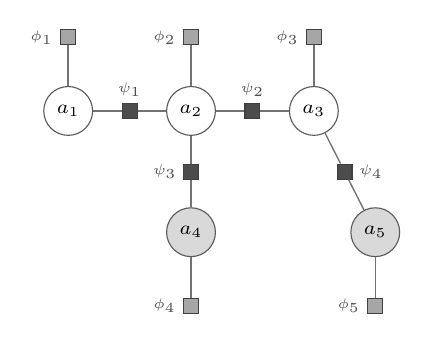
\begin{tikzpicture}[x=13mm, y=11mm]
  \node[atomtrue]  (a1) at (0,0)       {$a_1$};
  \node[atomtrue]  (a2) at (1.2,0)     {$a_2$};
  \node[atomtrue]  (a3) at (2.4,0)     {$a_3$};
  \node[atomfalse] (a4) at (1.2,-1.4)  {$a_4$};
  \node[atomfalse] (a5) at (3.0,-1.4)  {$a_5$};
  \foreach \v/\x/\y/\lab in {a1/0/0.85/$\phi_1$, a2/1.2/0.85/$\phi_2$, a3/2.4/0.85/$\phi_3$,
                              a4/1.2/-2.25/$\phi_4$, a5/3.0/-2.25/$\phi_5$}{
    \node[unary] (u\v) at (\x,\y) {}; \draw[flink] (u\v) -- (\v);
    \node[prlab,left=0.5mm of u\v] {\lab};
  }
  \node[factor] (f1) at (0.6,0)     {}; \draw[flink] (a1) -- (f1) -- (a2);
  \node[factor] (f2) at (1.8,0)     {}; \draw[flink] (a2) -- (f2) -- (a3);
  \node[factor] (f3) at (1.2,-0.7)  {}; \draw[flink] (a2) -- (f3) -- (a4);
  \node[factor] (f4) at (2.7,-0.7)  {}; \draw[flink] (a3) -- (f4) -- (a5);
  \node[prlab,above=0.4mm of f1] {$\psi_1$};
  \node[prlab,above=0.4mm of f2] {$\psi_2$};
  \node[prlab,left=0.4mm of f3]  {$\psi_3$};
  \node[prlab,right=0.4mm of f4] {$\psi_4$};
\end{tikzpicture}

\smallskip
\footnotesize
\setlength{\tabcolsep}{3.5pt}
\begin{tabular}{@{}lllcccc@{}}
\toprule
Factor & Scope & Relation & $00$ & $01$ & $10$ & $11$ \\
\midrule
$\phi_{1,\dots,5}$ & $a_i$ & prior $\frac12$ & \multicolumn{4}{c}{$a_i{=}0$: $\frac12$,\ \ $a_i{=}1$: $\frac12$} \\
\midrule
$\psi_1$ & $(a_1,a_2)$ & \ent, $p{=}.90$ & $1$ & $1$ & $\mathbf{.10}$ & $1$ \\
$\psi_2$ & $(a_2,a_3)$ & \ent, $p{=}.85$ & $1$ & $1$ & $\mathbf{.15}$ & $1$ \\
$\psi_3$ & $(a_2,a_4)$ & \con, $p{=}.90$ & $1$ & $1$ & $1$ & $\mathbf{.10}$ \\
$\psi_4$ & $(a_3,a_5)$ & \con, $p{=}.85$ & $1$ & $1$ & $1$ & $\mathbf{.15}$ \\
\bottomrule
\end{tabular}
\caption{The coherence MRF of Response~A. Circles are claims, grey squares the prior factors
  $\phi_i(x_i)$, black squares the relation factors. Each $\psi_r$ (Eq.~\ref{eq:psi}) is listed
  over the joint values $(x_s,x_t)$ of its two claims; bold cells are its violated set $V(\tau)$,
  down-weighted to $1-p_r$.}
\label{fig:mrf-a}
\end{figure}


With relations and weights in hand, we turn them into evidence about which worlds are consistent
with the response. The model is a Markov random field (MRF) with one binary variable $x_i$ per claim
and two kinds of factor. A \emph{prior factor} $\phi_i(x_i)=\pi_i^{x_i}(1-\pi_i)^{1-x_i}$ per claim
gives its plausibility before any relation is considered; together they multiply to the prior
$\pi(x)=\prod_i\phi_i(x_i)$. A \emph{relation factor} $\psi_r$ per relation depends only on the truth
values $(u,v)\in\{0,1\}^2$ of the relation's two claims, and down-weights exactly the joint values
the relation rules out:
\begin{equation}
\psi_r(u,v)\;=\;
\begin{cases}
1-p_r & \text{if } (u,v)\in V(\tau_r),\\
1 & \text{otherwise}.
\end{cases}
\label{eq:psi}
\end{equation}
For an entailment $a_s\Rightarrow a_t$, for example, $\psi_r(1,0)=1-p_r$ and $\psi_r=1$ on the other
three cells; Figure~\ref{fig:mrf-a} lists every factor of Response~A this way. We also write
$\psi_r(x)$ for $\psi_r(x_{e_r})$. The joint distribution is the prior times the relation factors,
\begin{equation}
\begin{gathered}
\PR(x)=\frac{1}{Z_\R}\,\pi(x)\prod_{r\in\R}\psi_r(x_{e_r}),\\
Z_\R=\sum_{x\in\{0,1\}^n}\pi(x)\prod_{r\in\R}\psi_r(x_{e_r}).
\end{gathered}
\label{eq:mrf}
\end{equation}

Read directly, Eq.~\ref{eq:mrf} keeps each world's prior weight and multiplies it by $1-p_r$ for
every relation the world violates: a world that violates no relation keeps its prior weight, one
that violates an entailment of weight $0.9$ keeps a tenth of it, and with no relations $\PR=\pi$.

\paragraph{Reading the MRF as a set of checks.} The weights also have a simple probabilistic
meaning. Picture a candidate world, an assignment of true or false to every claim, drawn at random
from the prior. Each relation of the response then acts as an independent \emph{check} on it. If the
world breaks the relation, for example by making the premise of an entailment true and its
conclusion false, the check raises an alarm with probability $p_r$. If the world respects the
relation, the check never raises one. The weight $p_r$ is thus how reliably the relation catches a
world that breaks it.

Now keep only the worlds that pass every check. A world passes the check of relation $r$ with
probability $\psi_r(x_{e_r})$: $1$ if it respects $r$ and $1-p_r$ if it breaks it. The checks are
independent, so the world passes them all with probability $\prod_r\psi_r(x_{e_r})$. By Bayes' rule,
the distribution of the surviving worlds is the prior times this product, renormalized, which is
exactly $\PR$ in Eq.~\ref{eq:mrf}. The normalizer $Z_\R$ is the probability that a world drawn from
the prior passes all checks. In short, $\PR$ is what we should believe about the claims after
learning that no check raised an alarm, with each relation catching a violation with
probability $p_r$.

For example, take two claims with flat priors, so each of the four worlds has probability $\frac14$,
and one entailment $a_1\Rightarrow a_2$ with $p_r=0.9$. Only the world $(1,0)$ breaks it, and it
survives the check with probability $0.1$. Hence $Z_\R=\frac34+\frac14\cdot0.1=0.775$, the world
$(1,0)$ falls to $0.025/0.775\approx0.03$, and each of the other three rises to $0.25/0.775\approx0.32$.
As $p_r\to1$ the check never misses, $(1,0)$ is eliminated, and the relation becomes a hard
constraint.

A table $\psi$ over a pair $e$ is \emph{sign-definite} at $\xs$ if its value at $\xs_e$ is its
maximum or its minimum. Because $\psi_r$ takes only the values $1$ and $1-p_r$, it is sign-definite
at every $\xs$: maximal when $\xs$ satisfies $r$ and minimal when $\xs$ violates it. \S\ref{sec:why}
shows that this is what monotonicity under adding and deleting relations requires. The MRF itself does not depend on $\xs$; only the
score read from it does.

Figure~\ref{fig:mrf-a} shows the MRF of Response~A: five claims with flat priors, two entailment
factors that penalize a premise holding while its conclusion fails, and two contradiction factors
that penalize worlds in which a true claim and a false one both hold. A world drawn from the priors passes all
four checks with probability $Z_A=\vyAZ$. The committed world violates none of them, and its
probability rises from $\pi(\xs)=2^{-5}\approx\vyAPiX$ to $P_A(\xs)=\vyAPX$. Under B's relations
the same world falls to $P_B(\xs)=\vyBPX$, because it violates both of B's conflicts.

\subsection{The Coherence Order and the Score}
\label{sec:order}
\label{sec:score}

To state the requirement of \S\ref{sec:intro} precisely, we need to say when one relation graph
over the same claims and committed world is more coherent than another.

\begin{definition}[Coherence order]
\label{def:order}
An \emph{elementary improvement} of $\R$ adds a support, raises a support's weight, deletes a
conflict, or lowers a conflict's weight. $\R'\coh\R$ if $\R'$ is reached from $\R$ by finitely
many elementary improvements, and $\R'\scoh\R$ if at least one of them changes a weight by a
non-zero amount, counting an addition or a deletion as a change of the relation's weight from or
to $0$.
\end{definition}

Given the committed world, the order is deliberately minimal: it ranks only edits that add or
strengthen relations $\xs$ satisfies or remove or weaken relations $\xs$ violates, and it leaves
edits that improve one part of an argument and degrade another unordered. Arbitrary rewiring is
covered whenever each step improves, and retyping a conflict as a support is an improvement. The
order is canonical relative to $\xs$, not independent of it: under verdict polarity, adding an
entailment between two false claims is an improvement, because it holds in the committed world.
This is the sense in which the score measures agreement with the facts. With the order fixed, we ask four things of
a score.

\begin{definition}[Axioms]
\label{def:axioms}
For a fixed committed world, a coherence score $S(\R;\pi)$ should be
\textbf{(A1) monotone}: $\R'\scoh\R\Rightarrow S(\R')>S(\R)$ for every $\pi$;
\textbf{(A2) MRF-grounded}: a functional of $\PR$ and $\pi$, so graphs inducing the same
distribution score the same;
\textbf{(A3) neutral}: $S(\varnothing;\pi)$ does not depend on $\pi$; and
\textbf{(A4) tractable}: computable from standard inference queries.
\end{definition}

A2 makes a score invariant to presentation, such as reversing a symmetric relation or swapping
\sense{Precedence} for \sense{Succession}. It also has a consequence worth stating: relations on one
pair that contradict each other, such as an exclusion and an equivalence of equal weight, multiply
to a constant and leave $\PR$ unchanged, so a score satisfying A2 rates them as uninformative
rather than as incoherent; we list this as a limitation. A1 is the demanding axiom, because the edited relation can sit anywhere
in an arbitrary graph. The requirement suggests reading the MRF at the one world whose standing the
argument is about, and comparing its probability after the relations with its probability before.

\begin{definition}[Logical coherence score]
\label{def:score}
\begin{equation}
\LCS(\R)=\sigma\bigl(\operatorname{logit}\PR(\xs)-\operatorname{logit}\pi(\xs)\bigr),
\label{eq:lcs}
\end{equation}
with $\sigma$ the logistic function and $\operatorname{logit}u=\log\frac{u}{1-u}$.
\end{definition}

The difference of log-odds in Eq.~\ref{eq:lcs} is Good's \emph{weight of evidence}
\citep{good1950} that the relations give the committed world: in the check model of \S\ref{sec:mrf}
it is $\log P(E\mid\xs)/P(E\mid\text{not }\xs)$, with $E$ the event that no check raises an alarm,
also known as the log-likelihood-ratio measure of confirmation \citep{fitelson1999}. $\LCS$ is
therefore the probability of $\xs$ after the relations for a reader who started from even odds on
it. It lies in $(0,1)$, with three reference points (Figure~\ref{fig:lcs-range}). A
\emph{completely incoherent} response, whose relations rule out the committed world, has
$\LCS\to0$: $\PR(\xs)\to0$, as when $\xs$ violates conflicts of weight approaching $1$ that some
other world satisfies. A response whose relations neither confirm nor disconfirm $\xs$, including
one with no relations, has $\PR(\xs)=\pi(\xs)$ and $\LCS=\frac12$. A \emph{completely coherent}
response, whose relations force the committed world, has $\LCS\to1$: $\PR(\xs)\to1$, which requires
relations that rule out every other world. Entailments, equivalences and contradictions never rule
out the world in which every claim is false, so forcing $\xs$ also needs co-necessity or exclusion
relations. Without them, and when $\xs$ is not that world, $n$ claims with flat priors stay below
$\LCS=1-2^{-n}$, which is $31/32\approx0.97$ for five, the value approached when every world but
$\xs$ and the all-false one is ruled out.

% The range of the LCS: LCS = sigma(W), W = logit P_R(x*) - logit pi(x*), the weight of
% evidence the relations give the committed world. Anchors: 0 (x* ruled out), 1/2
% (uninformative), 1 (x* forced). Voyager points from numbers.tex.
\begin{figure}[t]
\centering
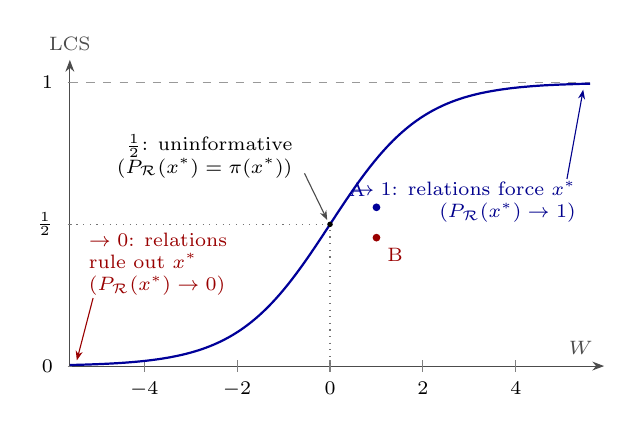
\begin{tikzpicture}[x=5.9mm,y=36mm,font=\scriptsize]
  % axes
  \draw[-{Stealth[length=1.5mm]},black!70] (-5.6,0) -- (5.9,0) node[above left=0.3mm] {$W$};
  \draw[-{Stealth[length=1.5mm]},black!70] (-5.6,0) -- (-5.6,1.08) node[above] {$\LCS$};
  \foreach \y/\l in {0/0, 0.5/\frac12, 1/1}
    \draw[black!50] (-5.65,\y) -- (-5.55,\y) node[left=1.2mm,text=black] {$\l$};
  \foreach \x in {-4,-2,0,2,4}
    \draw[black!50] (\x,-0.02) -- (\x,0.02) node[below=1.5mm,text=black] {$\x$};
  \draw[dashed,black!40] (-5.6,1) -- (5.6,1);
  \draw[dotted,black!55] (-5.6,0.5) -- (0,0.5) -- (0,0);
  % the curve
  \draw[thick,blue!60!black,domain=-5.6:5.6,samples=100,smooth]
       plot (\x,{1/(1+exp(-\x))});
  % anchors
  \node[anchor=west,align=left,text=red!60!black] at (-5.4,0.36)
       {$\to0$: relations\\rule out $\xs$\\($\PR(\xs)\to0$)};
  \draw[red!60!black,-{Stealth[length=1.2mm]}] (-5.1,0.24) -- (-5.45,0.02);
  \node[anchor=east,align=right] at (-0.6,0.74) {$\frac12$: uninformative\\($\PR(\xs)=\pi(\xs)$)};
  \draw[black!70,-{Stealth[length=1.2mm]}] (-0.55,0.68) -- (-0.06,0.515);
  \node[anchor=east,align=right,text=blue!55!black] at (5.5,0.58)
       {$\to1$: relations force $\xs$\\($\PR(\xs)\to1$)};
  \draw[blue!55!black,-{Stealth[length=1.2mm]}] (5.1,0.66) -- (5.45,0.975);
  \fill[black] (0,0.5) circle (1pt);
  % Voyager responses
  \fill[blue!60!black] (\vyAW,\vyALCS) circle (1.4pt) node[above left=0.2mm] {A};
  \fill[red!60!black] (\vyBW,\vyBLCS) circle (1.4pt) node[below right=0.2mm] {B};
\end{tikzpicture}
\caption{The range of the score. $\LCS=\sigma(W)$, where
$W=\operatorname{logit}\PR(\xs)-\operatorname{logit}\pi(\xs)$, the argument of $\sigma$ in
Eq.~\ref{eq:lcs}, is the weight of evidence the relations give the committed world. $\LCS$ tends to $0$ when the relations rule $\xs$ out, equals
$\frac12$ when they leave its probability at the prior, and tends to $1$ when they force it.
Responses A and B of Figure~\ref{fig:voyager} score $\vyALCS$ and $\vyBLCS$.}
\label{fig:lcs-range}
\end{figure}


\paragraph{Analysing the score.} The properties of $\LCS$ are easiest to state through the
log-ratio by which the relations raise the probability of the committed world,
\begin{align}
\Lambda(\R)&=\log\frac{\PR(\xs)}{\pi(\xs)}\notag\\
 &=\sum_{r\in\Rcon}\log(1-p_r)-\log Z_\R,
\label{eq:lambda}
\end{align}
where the second form holds because $\psi_r(\xs)$ is $1$ for a support and $1-p_r$ for a conflict.
Computing $\LCS$ therefore costs one query for the partition function $Z_\R$, exact by enumeration
for small claim sets and \#P-hard in general (\S\ref{sec:props}). In the check model $\Lambda$ is
the log-ratio measure of confirmation $\log P(\xs\mid E)/P(\xs)$ \citep{milne1996}, a different
measure from the weight of evidence in general \citep{fitelson1999}. Since
$\PR(\xs)=\pi(\xs)e^{\Lambda}$, however, $\LCS$ is a strictly increasing function of $\Lambda$ for
a fixed claim set and prior, so every ordering statement about $\Lambda$ holds for $\LCS$; we state
the results for $\Lambda$, where they take a closed form. The two differ in one respect. $\LCS$
depends on $\pi(\xs)$ and so on the whole claim set: adding a claim that no relation touches leaves
$\Lambda$ unchanged but moves $\LCS$ slightly towards $\sigma(\Lambda)$. The additivity and bounds
of \S\ref{sec:props} are therefore properties of $\Lambda$, not of $\LCS$. To see why the score
behaves well, consider adding a single relation.

\begin{lemma}[Edit identity]
\label{lem:edit}
For any $\R$, any relation $r$ and any priors,
$\Lambda(\R\uplus\{r\})-\Lambda(\R)=\log\psi_r(\xs)-\log\E_{\PR}[\psi_r]$. With
$q_r=\PR(x_{e_r}\in V(\tau_r))$, this is $-\log(1-p_rq_r)>0$ for a support and
$\log\frac{1-p_r}{1-p_rq_r}<0$ for a conflict (for $p_r>0$ and non-trivial $V(\tau_r)$, which
ensure $0<q_r<1$).
\end{lemma}

A relation's effect is its value at the committed world relative to its average under the current
model: its magnitude depends on the context, through $q_r$, but its sign does not. Since every
elementary improvement is a single addition, deletion or weight change, the main result follows.

\begin{theorem}[Monotonicity]
\label{thm:mono}
Fix $\xs$. For all priors $\pi\in(0,1)^n$ and all relation graphs $\R,\R'$ with weights in $[0,1)$:
if $\R'\coh\R$ then $\LCS(\R')\ge\LCS(\R)$, and if $\R'\scoh\R$ then $\LCS(\R')>\LCS(\R)$. The
same holds for $\Lambda$.
\end{theorem}

No interaction with other relations can reverse an improving edit, and the proof does not use
that scopes are pairs (App.~\ref{app:proof-score}). For edits the order leaves unranked,
Lemma~\ref{lem:edit} nets gains against costs. The Voyager pair is ranked by the theorem itself:
A is reached from B by deleting B's two conflicts and adding the supports $a_2\Rightarrow a_3$ and
$a_2\con a_4$, so $\R_A\scoh\R_B$. On Figure~\ref{fig:voyager}, A scores
$\LCS=\vyALCS$ ($\Lambda=\vyALam$) and B $\LCS=\vyBLCS$ ($\Lambda=\vyBLam$). The bars give each
relation's leave-one-out contribution to $\Lambda$ (\S\ref{sec:props}). B's two conflicts cost
$\vyBDTwo$ and $\vyBDThree$, far more than its supports earn. Magnitudes come from context, through
$q_r$. Both responses draw the same refutation $a_3\con a_5$, but it earns $\vyADFour$ in A and
only $\vyBDFour$ in B: B's conflict between $a_2$ and $a_3$ has already made $a_3$ less probable,
and with it the violating world in which $a_3$ and $a_5$ both hold, so the refutation has less left
to rule out.

\subsection{Why This Score}
\label{sec:why}

Theorem~\ref{thm:mono} rests on two choices, the potentials and the world at which the posterior is
read. We show that sign-definite tables are the only pairwise tables with the property, that the
readout world must be the world that defines the order, that a natural alternative readout fails,
and that the obvious simpler score fails too. The results are elementary; their value is in what
they rule out. First, is sign-definiteness merely sufficient, or is it needed?

\begin{theorem}[Sign-definiteness is necessary and sufficient]
\label{thm:necessity}
Fix the priors and $\xs$. Adding a positive table $\psi$ over a pair of claims $e$ never decreases
(resp.\ increases) $\Lambda$, for every relation graph, if and only if $\psi(\xs_e)=\max\psi$
(resp.\ $\min\psi$).
\end{theorem}

The theorem concerns adding and deleting relations; for weight changes, App.~\ref{app:proof-why}
gives the analogous sufficient condition. A natural alternative to Eq.~\ref{eq:mrf} uses tables that
are row-stochastic in the source, so that a false premise leaves its conclusion at the prior
(App.~\ref{app:earlier}). Such tables fail the test. At $\xs=\one$ they are sign-definite with the
intended sign only for $p\ge\frac12$; below it the committed cell of an entailment is the table's
minimum, so a weak entailment lowers the score and a weak contradiction raises it. When the
source is false at $\xs$, the committed cell holds the prior's value $\frac12$, which is neither the
maximum nor the minimum, so they fail at every weight except $p=\frac12$, where the table is
constant and has no effect. Second, the order of Def.~\ref{def:order}
is defined at $\xs$; could the score be read at another world?

\begin{proposition}[The readout world must define the order]
\label{prop:unique}
For $n\ge2$ and any world $x\neq\xs$, some elementary improvement strictly lowers
$\log\PR(x)-\log\pi(x)$, for any priors and any $\R$.
\end{proposition}

The proposition does not say that $\xs$ is the right world; choosing it is the factuality
pipeline's job. It says that the order and the readout must use the same world, so a score
monotone in agreement with the verdicts has to be read at the verdicts.

Third, could an average of beliefs replace a single world? The natural candidate is the mean
posterior marginal.

\begin{proposition}[The mean marginal is not monotone]
\label{prop:mm}
There are graphs in which deleting a contradiction strictly lowers the mean marginal
$\frac1n\sum_i\PR(a_i{=}1)$, under Eq.~\ref{eq:mrf} and row-stochastic tables alike.
\end{proposition}

\label{sec:failures}
In the witness, a contradiction holds down a hub claim that itself contradicts five others;
deleting it releases the hub, and the mean marginal falls from $\starFiveMMa$ to $\starFiveMMb$
while $\Lambda$ rises. The failure is not rare. Over \thmSteps{} random improving edits at
$\xs=\one$, the mean marginal falls on \fallsPctMmSigndef\% and Shogenji's coherence measure \citep{shogenji1999} on
\fallsPctShogenjiSigndef\%, while $\Lambda$ never does (App.~\ref{app:verify}).

These results fix the class of tables and the readout world; they do not make $\Lambda$ the unique
score satisfying A1--A4. Any score that is strictly increasing in $\Lambda$ for a fixed prior and
takes a prior-independent value at $\Lambda=0$ satisfies them too, which is how $\LCS$ does. And any
reweighting $p\mapsto1-(1-p)^\beta$ with $\beta>0$ gives another monotone score of the same form,
where different $\beta$ can rank incomparable graphs differently. We take $\beta=1$ because it makes $p_r$ the
probability that a check catches a violation, so that the check reading of
\S\ref{sec:mrf} holds with the weights as estimated.

\paragraph{Why not count relations?} Monotonicity alone admits trivial scores: the signed weight sum
$\sum_{\Rsup}p_r-\sum_{\Rcon}p_r$ is monotone by construction. But a count credits every relation
in full, whether or not it rules out anything plausible, so it depends on how an argument is
presented rather than on what it rules out. Two entailments $a\Rightarrow b$ and $b\Rightarrow a$ of
weight $p$ multiply to exactly the table of one equivalence of weight $p$, so they induce the same
$\PR$ and the same $\Lambda$, but they count $2p$ against $p$, which violates A2. Repeating a
support likewise adds its weight each time, where $\Lambda$ saturates (Prop.~\ref{prop:sat}).
Averaging removes the dependence on the number of relations but breaks monotonicity, since a weak
support lowers an average. $\Lambda$ weighs each relation by what it rules out under the rest of the
model (Lemma~\ref{lem:edit}), which is what the MRF contributes.

\subsection{Further Properties}
\label{sec:props}

Four structural properties follow, from the edit identity, the factorization of $\PR$ and a
relabelling of worlds.

\begin{proposition}[Neutrality, sign and additivity]
\label{prop:basic}
(i) $\Lambda(\varnothing)=0$ for every $\pi$. (ii) $\Lambda\ge0$ if $\R$ has only supports and
$\Lambda\le0$ if only conflicts. (iii) If $\R_1$ and $\R_2$ have scopes in disjoint sets of
claims, $\Lambda(\R_1\uplus\R_2)=\Lambda(\R_1)+\Lambda(\R_2)$.
\end{proposition}

Additivity makes $\Lambda$ an amount of evidence, in nats, that adds across independent parts of an
argument; $\LCS$, a transform of $\Lambda$ that depends on the claim set, is not additive. The score
also does not depend on how the decomposition phrases a claim.

\begin{proposition}[Negation invariance]
\label{prop:neg}
Replace a claim $a_i$ by $\neg a_i$, setting $\xs_i\mapsto1-\xs_i$ and $\pi_i\mapsto1-\pi_i$ and
rewriting each coupling at $a_i$ by negating that endpoint. Every relation keeps its sign and its
weight, and $\Lambda$ and $\LCS$ are unchanged.
\end{proposition}
Monotonicity in supports raises
the question of padding: if supports never hurt, can a response gain without bound by adding them?

\begin{proposition}[Bounds and saturation]
\label{prop:sat}
(i) $\sum_{r\in\Rcon}\log(1-p_r)\le\Lambda(\R)\le-\log\pi(\xs)$. (ii) A support's gain is at most
$-\log\bigl(1-p_r(1-\PR(\xs))\bigr)$. (iii) A second copy of a support adds strictly less than the
first.
\end{proposition}

A support earns credit only for the probability it removes from worlds other than $\xs$, so once
the relations force $\xs$, further support earns almost nothing; repeated copies of one relation
converge rather than accumulate (App.~\ref{app:proof-props}). Finally, the leave-one-out
contribution $\Delta_r=\Lambda(\R)-\Lambda(\R\setminus\{r\})$ of every relation has a guaranteed
sign, which localizes what costs an argument most (the bars of Figure~\ref{fig:voyager}). The
contributions are not additive and need not sum to $\Lambda$. $\Lambda$ and each $\Delta_r$ cost
one partition-function query, which is \#P-hard in general. It is exact by enumeration for
$n\le20$, and by variable elimination when the relation graph has low treewidth; beyond that it is
approximated by weighted mini-bucket elimination \citep{wmb}, where the guarantees hold only up to
the approximation.

%% ================================================================
\section{Evaluation Data}
\label{sec-locobench}
%% ================================================================

Testing the requirement of \S\ref{sec:intro} needs responses that differ in argument structure
while their claims stay fixed, together with gold relation graphs that say what each response
argues. Natural corpora do not provide this: two documents that differ in coherence almost always
differ in topic, length and claims as well. We therefore evaluate on \textsc{LoCoBench}
\citep{anonlocobench}, a synthetic benchmark of \emph{coherence ladders} introduced in a companion
paper; we use it here and summarize what is needed to read our results
(App.~\ref{sec-full-locobench}). A ladder is a family of five responses, its \emph{rungs}, built
from the same claims and topic and differing along a single structural dimension. Each rung carries
its own gold relation graph, and the family declares how the rungs' scores must be ordered. Because
the gold graphs are given, a coherence measure can be evaluated separately from relation
extraction.

\paragraph{Four ladder types.} \cp{conflict} ladders add spurious contradictions on their lower
rungs and resolve conceded tensions on their upper rungs, so coherence increases strictly from
bottom to top. \cp{chain} ladders break links of an entailment chain on their lower rungs and drop
a conflict on their top rung, testing sensitivity to \emph{missing} support rather than only to a
present contradiction. \cp{order} ladders reorder sentences and \cp{control} ladders reverse
symmetric relations or swap temporal senses; neither changes any factor of the relation graph, so
both require identical scores throughout. Together they separate coherence measures from metrics
that track contradictions only, surface edits, or length.

\paragraph{The development split.} Each family is generated by a model from a declared relation
plan and admitted only if a committee of models from other vendors recovers the planned relations
from the prose and finds every planned claim asserted. We use the repaired development split of
the companion paper, in which every perturbed rung was additionally gated on realizing its planned
change; five \cp{conflict} families whose planted change could not be realized were excluded,
leaving \devFamilies{} families (\devItems{} responses, \devRelations{} gold relations). Two
dependencies matter for reading mined results: admission required relation recovery by the same
prompt our graph-level miner uses, and the generator and one miner belong to the same model family.
A pilot human study in the companion paper, run before the repair, found that readers reproduce
the declared increases and judge \cp{control} rungs equal, but distinguish reordered \cp{order}
rungs on grounds of discourse rather than logical coherence. \cp{order} invariance therefore marks
the scope of a logical-coherence score, not a claim that sentence order never matters.

%% ============================================================================
\section{Experiments}
\label{sec:experiments}
\label{sec-experiments}
%% ============================================================================

The theory makes three predictions that can be checked on LoCoBench. On gold relation graphs,
where every rung transition is an elementary improvement or a presentation change, the score
should satisfy every ordering and every invariance the ladders declare. On mined graphs, where no
guarantee applies, every error should trace back to the extracted relations rather than to the
score. And verdict polarity should change the result only where a relation's truth differs from
its assertion. We test each in turn, after fixing the setup.

\subsection{Setup}
\label{sec:exp-setup}

\paragraph{Data and assertions.} We use the repaired development split of LoCoBench
(\S\ref{sec-locobench}): \devFamilies{} families and \devItems{}
responses of \devAtomsMin--\devAtomsMax{} claims, with \devRelations{} gold relations. Each claim's
factuality label serves as its verdict, so $\xs_i=1$ for a claim labelled true and $0$ otherwise,
with flat priors (\S\ref{sec:setup}). Within a family all $\binom52=10$ rung pairs are ordered.
A \cp{conflict} or \cp{chain} pair is satisfied by a strict increase ($>10^{-9}$, exact
arithmetic), giving 50 \emph{Increase} assertions; an \cp{order} or \cp{control} pair by equality
to within $10^{-9}$, giving 40 \emph{Invariance} assertions. The ladders were designed around the
claims as asserted, so their declared orderings are the coherence order at $\xs=\one$.

\paragraph{Arms and scores.} An \emph{arm} fixes where the relation graph comes from and holds the
claims, priors and scorer identical, so arms differ only in the relation graph. \cp{gold} compiles
each response's labelled relations, weighted at the midpoint of the labelled strength band. Three
\cp{mined} arms run the graph-level miner of \S\ref{sec:mining} with Claude Opus~5.5, GPT-6.1 and
gpt-oss-120b; arms using the pairwise miner are \tbd{to be run on the repaired split}. We report
$\Lambda$ under verdict polarity (the default) and under assertion polarity. As a reference we
report the mean posterior marginal over the row-stochastic tables of App.~\ref{app:earlier}, the natural
readout of a claim MRF and one that is not monotone (Prop.~\ref{prop:mm}), with that model's priors
($0.9$ for claims labelled true, $0.1$ otherwise). All scores are computed exactly on the same
graphs, and every number is regenerated from the data by one script.

\begin{table*}[t]
\centering\small
\setlength{\tabcolsep}{5pt}
\begin{tabular}{@{}lcccccccc@{}}
\toprule
& \multicolumn{2}{c}{\cp{gold}} & \multicolumn{2}{c}{Claude Opus 5.5}
& \multicolumn{2}{c}{GPT-6.1} & \multicolumn{2}{c}{gpt-oss-120b} \\
\cmidrule(lr){2-3}\cmidrule(lr){4-5}\cmidrule(lr){6-7}\cmidrule(l){8-9}
Score & Incr. & Inv. & Incr. & Inv. & Incr. & Inv. & Incr. & Inv. \\
\midrule
Mean marginal (not monotone) & \ladGoldMMIncAll & \ladGoldMMInvAll & \ladOpusMMIncAll & \ladOpusMMInvAll
  & \ladGptMMIncAll & \ladGptMMInvAll & \ladOssMMIncAll & \ladOssMMInvAll \\
$\Lambda$, assertion polarity ($\xs=\one$) & \ladGoldConfAIncAll & \ladGoldConfAInvAll
  & \ladOpusConfAIncAll & \ladOpusConfAInvAll
  & \ladGptConfAIncAll & \ladGptConfAInvAll & \ladOssConfAIncAll & \ladOssConfAInvAll \\
$\Lambda$, verdict polarity (ours) & \ladGoldConfIncAll & \ladGoldConfInvAll
  & \ladOpusConfIncAll & \ladOpusConfInvAll
  & \ladGptConfIncAll & \ladGptConfInvAll & \ladOssConfIncAll & \ladOssConfInvAll \\
\midrule
LLM judge (G-Eval) & \multicolumn{2}{c}{---} & \multicolumn{6}{c}{\tbd{re-run on the repaired dev split}} \\
\bottomrule
\end{tabular}
\caption{Ladder assertions satisfied on the LoCoBench development split (all 10 rung pairs per
family; 50 Increase, 40 Invariance). The mean marginal over row-stochastic tables is the
non-monotone reference. Exact enumeration. Per-ladder breakdowns are in
App.~\ref{app:results}.}
\label{tab:ladders}
\end{table*}

\subsection{Gold Graphs: The Theorem, Observed}
\label{sec:exp-gold}

Under assertion polarity, Theorem~\ref{thm:mono} predicts $50/50$ Increase and A2 predicts $40/40$
Invariance, and Table~\ref{tab:ladders} confirms both. Under verdict polarity, exactly one gold edit
changes sign. A \cp{conflict} rung deletes a spurious contradiction between two claims that are
both labelled \emph{false}. ``These two cannot both hold'' is true of two falsehoods, so relative
to $\xs$ the deleted relation was a support, the pair is ordered \emph{backwards}, and $\Lambda$
falls, as the theorem requires. This is the one place where the ladder's design (the internal
coherence of what is asserted) and verdict polarity (how well the claims, as they stand, support
one another) disagree, and the disagreement is principled. On the \domGoldForward{} gold pairs that
are ordered relative to $\xs$, and on the \domGoldIncomparable{} pairs that span the reversed edit,
$\Lambda$ is right every time (Table~\ref{tab:dominance}).

The mean marginal misses the same pair, for a different reason: under the row-stochastic
table the deleted contradiction was \emph{raising} its source's marginal ($0.096\to0.125$) by more
than it lowered its target's ($0.099\to0.091$). That is an artefact of the tables rather than a
principled reversal, and Prop.~\ref{prop:mm} shows the mean marginal can fall on genuine
improvements too.

\subsection{Mined Graphs: Separating Estimation from Scoring}
\label{sec:exp-mined}

On mined graphs no score is guaranteed anything, because a miner changes relations in both
directions at once. We can still ask, pair by pair, whether the miner's two graphs are ordered as
the ladder says (Def.~\ref{def:order} relative to $\xs$, with parallel relations merged), and
Table~\ref{tab:dominance} splits the Increase pairs accordingly. Wherever the extracted graphs are
correctly ordered, $\Lambda$ is right on every pair, for every miner, as Theorem~\ref{thm:mono}
requires. Every error falls on a pair whose extracted graphs are \emph{incomparable}, where the
miner added a spurious support or dropped a real one between the two rungs. The weaker the miner,
the more pairs it leaves incomparable: \domOpusIncomparable{} for Opus~5.5 (coupling F1
\extOpusCouplingFOne), \domGptIncomparable{} for GPT-6.1 (\extGptCouplingFOne) and
\domOssIncomparable{} for gpt-oss-120b (\extOssCouplingFOne). The remaining errors are errors of
relation estimation, not of the score.

\begin{table}[t]
\centering\small
\setlength{\tabcolsep}{3.5pt}
\begin{tabular}{@{}lcccc@{}}
\toprule
Arm & F1 & Ordered & Incomp. & Backward \\
\midrule
\cp{gold} & --- & \domGoldForwardOk/\domGoldForward & \domGoldIncomparableOk/\domGoldIncomparable
  & \domGoldBackwardOk/\domGoldBackward \\
Opus 5.5 & \extOpusCouplingFOne & \domOpusForwardOk/\domOpusForward
  & \domOpusIncomparableOk/\domOpusIncomparable & --- \\
GPT-6.1 & \extGptCouplingFOne & \domGptForwardOk/\domGptForward
  & \domGptIncomparableOk/\domGptIncomparable & --- \\
gpt-oss-120b & \extOssCouplingFOne & \domOssForwardOk/\domOssForward
  & \domOssIncomparableOk/\domOssIncomparable & --- \\
\bottomrule
\end{tabular}
\caption{Increase pairs by how the two rungs' graphs compare in the coherence order relative to
$\xs$ (verdict polarity), and the pairs $\Lambda$ satisfies in each class. ``Ordered'': the higher
rung's graph dominates the lower rung's; on a ``backward'' pair the theorem requires $\Lambda$ to
\emph{fall}. F1 is coupling-level extraction F1. One Opus pair has identical mined graphs.}
\label{tab:dominance}
\end{table}

On incomparable pairs no score has a guarantee, and the mean marginal is close to $\Lambda$ on the
two strong miners; with \devFamilies{} families we do not read differences there as more than that.
What separates $\Lambda$ is that it is guaranteed to be right on every pair the miner orders
correctly. Invariance on mined graphs is low for every score for the same reason: a resampled miner
returns a slightly different graph for a reordered text, and A2 promises nothing about a graph that
has changed. The median $|\Delta\LCS|$ on mined Invariance pairs, \sprOpusInv{} for Opus~5.5 and
\sprGptInv{} for GPT-6.1, is well below the median Increase step (\sprOpusInc, \sprGptInc), so a
tolerance-based invariance test is meaningful for strong miners; we leave its calibration to the
repaired split.

\subsection{What Polarity Changes}
\label{sec:exp-polarity}

Verdict polarity matches or raises the mined Increase counts of assertion polarity on every miner,
most where extraction is noisiest: \ladOssConfIncAll{} against \ladOssConfAIncAll{} for
gpt-oss-120b. The reason is the sign rule of Table~\ref{tab:couplings}. A spurious relation that a
miner draws between a true and a false claim changes sign with the committed world: a
contradiction between the two counts as the argument rejecting a falsehood rather than as a
self-contradiction of the response. On gold graphs the two polarities differ only on the single
edit discussed above. The polarity thus changes the score exactly where a relation's truth and its
assertion come apart, and nowhere else.

%% ============================================================================
\section{Discussion}
\label{sec:discussion}
%% ============================================================================

The results raise three questions about what the score is for: what its guarantee covers, how it
divides the work with factuality evaluation, and what it deliberately leaves out.

\paragraph{What the guarantee covers.} Theorem~\ref{thm:mono} is a statement about the map from
relation graphs to scores, not about the graphs themselves. It guarantees that the score never
misranks two responses whose relations are ordered. Observing this on mined graphs is a check of
the implementation rather than new evidence, but it is useful: it confines every ranking error to
pairs whose extracted graphs are incomparable, where any score must choose how to net gains against
costs and a different monotone score might choose differently. No learned or judge-based score
offers even this much. The guarantee does not make relation extraction easier; it marks extraction
as the place where improvements will show.

\paragraph{Coherence given the facts.} With verdict polarity, factuality and coherence evaluation
divide the work, and the interface between them is a verdict per claim, together with its
posterior when the pipeline provides one. Any factuality pipeline decides which claims are true; the coherence score asks how well the relations the response draws
hold up under that verdict. The verdicts decide the sign of each relation, crediting refutations of
falsehoods and charging denials of truths and derivations of falsehoods from truths, while the
magnitude of each relation's effect comes from what it rules out under the rest of the argument.
It does not penalize a response for asserting false claims, which is the factuality score's job:
keeping the two separable is deliberate, and the two scores can be reported side by side.
Without a factuality stage, assertion polarity gives the internal-coherence reading, and the two
polarities disagree exactly where a relation's truth differs from its assertion, as in the gold
edit of \S\ref{sec:exp-gold}.

\paragraph{What the score leaves out.} The score measures \emph{logical} coherence, the fit between
a response's claims and the truth-functional relations it draws between them. It is blind to
discourse coherence: readers in the human study (\S\ref{sec-locobench}) preferred unshuffled
\cp{order} rungs that the score, correctly by its own definition, rates as equal. It also
compares responses only over a fixed claim set and committed world, which is the setting of the
requirement but not of every evaluation; ranking responses with different claims requires a
choice of normalization that the theory does not make. The Limitations section lists the
remaining caveats.

%% ============================================================================
\section{Related Work}
\label{sec:related}
%% ============================================================================

\paragraph{Factuality and the logic gap.} Claim-level metrics such as FActScore \citep{factscore},
SAFE \citep{safe} and VeriScore \citep{veriscore} aggregate independent per-claim verdicts, and
FactReasoner \citep{factreasoner} replaces counting with inference over claims and retrieved
evidence. \citet{lorefact} identify the resulting logic gap and label inter-claim dependencies as a
classification task. We take the verdicts of such a pipeline as input and score the relations
between claims, rather than the claims themselves.

\paragraph{Consistency and reasoning evaluation.} NLI-based detectors flag inconsistencies between a
summary and its source \citep{summac}, across sampled generations \citep{selfcheckgpt} and within
one generation \citep{mundler2024}, and probes measure the consistency of a model's beliefs
\citep{elazar2021}. Reasoning-chain metrics score explicit step-by-step derivations by step-wise
entailment and informativeness \citep{roscoe,receval}, and are evaluated, among others, on
entailment trees \citep{entailmentbank}. These methods detect conflicts or score explicit chains; they do not say
how a response's supports and conflicts should combine, and none has a notion of a committed world
under which refuting a falsehood counts as support.

\paragraph{Discourse coherence.} Entity grids \citep{barzilay}, neural coherence models \citep{li},
DiscoScore \citep{discoscore} and entity--discourse graphs \citep{liustrube} score coherence from
surface statistics, learned representations or discourse relations \citep{pdtb,mann}, and LLM
judges are the practical incumbent \citep{geval,zheng2023judge}. These methods measure cohesion and
organization rather than truth-functional constraints between claims, and none guarantees how its
score responds to a change in those constraints.

\paragraph{Argumentation.} Argument mining recovers support and attack relations from text
\citep{stab2017}, and argument-quality frameworks rate dimensions such as cogency
\citep{wachsmuth2017}. Gradual semantics for weighted bipolar argumentation assign acceptability
degrees to arguments under axioms such as neutrality, monotony and reinforcement
\citep{cayrol2005,amgoud2016,amgoud2018,baroni2019}, the closest precedent to our axioms.
Probabilistic argumentation puts a distribution over arguments, or over the worlds in which they
are accepted, and constrains it by attacks \citep{thimm2012,hunter2013}, and explanatory coherence
treats coherence as the satisfaction of positive and negative constraints
\citep{thagard1989,thagard1998}. Our setting differs in three ways: relations are truth-functional
couplings between claims rather than attacks between arguments, a relation's sign is fixed by the
factuality verdicts rather than by its type, and monotonicity is asked of a readout of one
probability model, so that what must be justified is the choice of potentials and of the world the
readout uses.

\paragraph{Logical constraints over claims.} Our couplings are the basic relations of natural logic
\citep{maccartney2009}. BeliefBank \citep{beliefbank}, ConCoRD \citep{concord} and Maieutic prompting
\citep{maieutic} use weighted MAX-SAT or factor-graph inference over NLI constraints to make a
model's beliefs consistent, and Markov logic \citep{mln} and probabilistic soft logic \citep{psl}
are general frameworks for weighted logical constraints. We use the same kind of model to
\emph{measure} a response rather than correct it. That raises a question these methods do not face:
which readout of the model is monotone in its constraints.

\paragraph{Probabilistic coherence and confirmation.} Bayesian epistemology measures the coherence
of a set of propositions under a joint distribution, for example as the ratio of their joint
probability to the product of their marginals \citep{shogenji1999}. Alternatives come from
\citet{olsson2002}, \citet{fitelson2003} and \citet{douven2007}, and \citet{bovens2003} prove
impossibility results on truth-conduciveness. Confirmation theory measures how evidence moves
belief in a hypothesis. Among its standard measures are the log-ratio, which \citet{milne1996}
argues is canonical, and the log-likelihood ratio, Good's weight of evidence \citep{good1950}; they
are not ordinally equivalent in general \citep{fitelson1999,crupi2007}. $\LCS$ is a monotone
transform of the weight of evidence, with the committed world as the hypothesis and the event that
the response's relations hold as the evidence, and $\Lambda$ is the log-ratio measure; for a fixed
claim set and prior the two order relation graphs identically. Unlike coherence measures, ours
holds the propositions fixed and varies the relations, and we show that Shogenji's measure is not
monotone in that setting.

%% ============================================================================
\section{Conclusion}
%% ============================================================================

We asked what a coherence score over a response's own relations must guarantee and answered with
a single requirement, monotonicity in the coherence order over a fixed claim set. The score that
meets it is the weight of evidence that the coherence MRF lends to the committed world: the claims, with
the truth values a factuality pipeline assigns them. It is strictly monotone in every context;
among pairwise tables, sign-definiteness is exactly what monotonicity in additions and deletions
requires; and the score must be read at the world that defines the order. Its log-ratio form is
neutral, additive and saturating. On the benchmark it behaves as the theory
predicts, and its errors on declared increases in mined graphs are confined to pairs the miner left
incomparable, which makes relation extraction the open problem.

\section*{Limitations}

\textbf{Data.} The evaluation uses a small development split (\devFamilies{} families,
\devItems{} responses) generated by a single model family and is still being repaired; five
\cp{conflict} families were excluded because their planted spurious link could not be realized
in prose. Its ladders encode internal coherence of the asserted claims, which verdict polarity
reorders on one pair. Baselines outside the MRF (LLM judges, NLI contradiction rates, discourse
metrics) have to be re-run on the repaired split and are marked as pending. Human judgments of
coherence are not yet collected for this split.
\textbf{Realism of the benchmark.} LoCoBench is a diagnostic benchmark, not a sample of how real
responses argue. Its prose is expert in register and its relations are recoverable by blind
readers, but its structure is engineered: every plan has ten relations, six valid and four
planted-invalid, two or more false claims, and a quota of rare senses, so that every dev base
response contains an exhaustive alternative and a disjunction, usually signalled by explicit
markers (``at least one of\dots{} perhaps both'', ``exactly one''). Rungs differ by single minimal
edits along one dimension, spurious links are sometimes realized by contrived constructions, and
claims are given rather than extracted, so atomization errors are absent. The benchmark therefore
tests whether a score satisfies the orderings its theory predicts and separates extraction errors
from scoring errors; it does not measure agreement with human coherence judgements on natural
responses, or how often incoherence occurs in practice. Because relations are explicitly marked,
mined-graph results are best read as upper bounds on extraction from natural text. An evaluation on
natural responses with human coherence ratings is needed to establish external validity.
\textbf{Selection.} Families were admitted only if a committee model recovered their relations with
the same prompt our graph-level miner uses, and the generator and one miner share a model family,
so mined results on this corpus are optimistic.
\textbf{Scope of the guarantee.} Monotonicity is with respect to the relation graph, for a fixed
committed world. When an extractor changes relations in both directions, the score nets them and
no ordering is guaranteed. The score does not compare responses with different claim sets, and
its necessity results fix the tables and the readout world but not the functional form of the
score. Relations on
one pair that contradict each other cancel and score as uninformative rather than as incoherent.
$\LCS$ also shifts slightly when claims without relations are added, so across claim sets it is a
reading on a common scale rather than a guaranteed order.
\textbf{Polarity.} Verdict polarity inherits the factuality pipeline's errors: a wrong verdict
can flip the sign of the relations at that claim. Verdicts are binary, so a claim the evidence
neither supports nor refutes is treated as false. With a probabilistic pipeline the score
also inherits the calibration of its posteriors, which set how much each relation counts
(App.~\ref{app:twostage}); with a label-only pipeline it uses no confidence at all. Assertion
polarity assumes the decomposition records the response's stance on each claim, or records a
denied claim as its negation (Prop.~\ref{prop:neg}).
\textbf{Modelling.} Relation weights in the gold arm are band midpoints and, in the mined arms,
existence shares times band midpoints; neither is calibrated. Only \sense{Refutation} compiles to
\con{}, so an incompatibility the response conveys without asserting it, for instance through a
bare contrast, produces no factor; separating asserted incompatibility from contrast is left to the
miner. Couplings are material constraints: an entailment from a false premise is upheld whatever
its conclusion, and so is credited as a support, and relevance of premise to conclusion is not
modelled. The proofs extend to relations over more than two claims (App.~\ref{app:proofs}), but the
definitions and experiments are pairwise. Saturation bounds the effect of redundant
support but cannot stop a miner from hallucinating new support, so the score inherits the
extractor's precision.

\section*{Ethics Statement}

The score is intended for evaluating and diagnosing generated text. A high coherence score is not
evidence of truth, and should not be used on its own to certify content. The corpus is synthetic
and contains no personal data. By design it contains plausible false claims written as expert prose
without hedging; every item carries per-claim factuality labels, and released copies should keep
them attached so that the false claims are not reused as fact. The responses were generated by
commercial models and are released under those providers' terms for research use. The human
studies on the benchmark are reported, with their ethics provisions, in the companion paper; this
paper collects no new human data. LLMs were used to generate the benchmark
responses and to extract relations, as described; they were also used for editing assistance in
preparing this paper.

\bibliography{ref}

\appendix

%% ============================================================================
\section{Proofs}
\label{app:proofs}
%% ============================================================================

Throughout, $\xs$ is a fixed committed world, priors lie in $(0,1)$ and weights in $[0,1)$, so
every world has positive mass under every $\PR$. For a scope $e$ write $V\subseteq\{0,1\}^{|e|}$
for a violated set with $\varnothing\ne V\ne\{0,1\}^{|e|}$; a relation with $V=\varnothing$ or
$V=\{0,1\}^{|e|}$ contributes a constant factor and leaves $\PR$ unchanged.

\subsection{The Score (\S\ref{sec:score})}
\label{app:proof-score}

\paragraph{Lemma~\ref{lem:edit}.} Let $\tilde P(x)=\pi(x)\prod_{r'\in\R}\psi_{r'}(x)$, so
$\PR=\tilde P/Z_\R$. After adding $r$, the unnormalized mass is $\tilde P\psi_r$, with normalizer
$Z_{\R\uplus\{r\}}=\sum_x\tilde P(x)\psi_r(x)=Z_\R\,\E_{\PR}[\psi_r]$. Hence
$P_{\R\uplus\{r\}}(\xs)=\PR(\xs)\psi_r(\xs)/\E_{\PR}[\psi_r]$; taking logarithms and subtracting
the constant $\log\pi(\xs)$ gives the identity. For $\psi_r$ of Eq.~\ref{eq:psi},
$\E_{\PR}[\psi_r]=1-p_rq_r$ with $q_r=\PR(x_{e_r}\in V(\tau_r))\in(0,1)$, and $\psi_r(\xs)$ is $1$ for a
support and $1-p_r$ for a conflict, which gives the two closed forms and their signs. $\square$

\paragraph{Theorem~\ref{thm:mono}.} By transitivity it suffices to show that each elementary
improvement does not decrease $\Lambda$, and strictly increases it when it changes a weight by a
non-zero amount. Fix the improvement and let $\R_0$ be the graph without the edited relation $r$
(for an addition, the graph before; for a deletion, the graph after). Write
$q=P_{\R_0}(x_e\in V)$; by positivity and the non-triviality of $V$, $0<q<1$. Define
$g(p)=\Lambda(\R_0\uplus\{(e,\tau,p)\})-\Lambda(\R_0)$. By Lemma~\ref{lem:edit},
$g^+(p)=-\log(1-pq)$ for a support and $g^-(p)=\log(1-p)-\log(1-pq)$ for a conflict, with
$g^\pm(0)=0$, and
\begin{gather*}
\tfrac{d}{dp}g^+=\tfrac{q}{1-pq}>0,\\
\tfrac{d}{dp}g^-=-\tfrac{1-q}{(1-p)(1-pq)}<0\quad\text{on }[0,1).
\end{gather*}
(i) Adding a support of weight $p>0$ changes $\Lambda$ by $g^+(p)>0$. (ii) Raising a support's
weight from $p$ to $p'>p$ changes it by $g^+(p')-g^+(p)>0$. (iii) Deleting a conflict of weight
$p>0$ changes it by $-g^-(p)>0$. (iv) Lowering a conflict's weight from $p$ to $p'<p$ changes it
by $g^-(p')-g^-(p)>0$. A zero-weight addition or deletion leaves $\Lambda$ unchanged. Parallel
copies of the edited relation are part of $\R_0$, so multisets are handled. $\LCS$ is a strictly
increasing function of $\Lambda$ for a fixed claim set and prior, which gives the statement for
$\LCS$. Nothing in the argument uses $|e|=2$, and $\xs$
enters only through which relations are supports, that is, through $\psi_r(\xs)\in\{1,1-p_r\}$.
$\square$

\paragraph{A three-claim example by hand.} Take three claims, all verified true, at $\pi_i=\frac12$ (so $\xs=\one$
under either polarity), with $a_1\Rightarrow a_2$ and $a_2\Rightarrow a_3$ at weight $0.9$ and a
contradiction between $a_1$ and $a_3$ at $0.8$ (Table~\ref{tab:worked}). With only the chain, the
violating worlds are those with $(a_1,a_2)=(1,0)$ or $(a_2,a_3)=(1,0)$; no world violates both,
since that would need $a_2=0$ and $a_2=1$. The unnormalized masses ($\times8$) are
$1,1,0.1,1,0.1,0.1,0.1,1$ for $x=000,\dots,111$, summing to $4.4$, so
$\PR(\one)=1/4.4=\wkChainP$, $\Lambda=\log(8/4.4)=\wkChainLam$, and
$\PR(a_1{=}a_3{=}1)=1.1/4.4=\wkPOneThree$. Adding the contradiction therefore costs exactly
$\log\frac{0.2}{1-0.8\cdot\wkPOneThree}=\wkConflictGain$, as Lemma~\ref{lem:edit} predicts.
Weakening it to $0.44$ recovers most of the loss. The posterior marginals under the chain
are $(0.295,0.500,0.705)$: sign-definite entailments lower the premise's marginal, one more reason
the score is not a function of the marginals.

\begin{table}[h]
\centering\small
\setlength{\tabcolsep}{5pt}
\begin{tabular}{@{}lccc@{}}
\toprule
Relations & $\PR(\one)$ & $\Lambda$ & $\LCS$ \\
\midrule
none (bag of claims)          & \wkBagP & \wkBagLam & \wkBagLCS \\
contradiction only           & \wkConflictP & \wkConflictLam & \wkConflictLCS \\
chain                        & \wkChainP & \wkChainLam & \wkChainLCS \\
chain + contradiction         & \wkChainConflictP & \wkChainConflictLam & \wkChainConflictLCS \\
chain + weakened contradiction & \wkChainResolvedP & \wkChainResolvedLam & \wkChainResolvedLCS \\
\bottomrule
\end{tabular}
\caption{Three claims, uniform priors, exact values.}
\label{tab:worked}
\end{table}

\subsection{Why This Score (\S\ref{sec:why})}
\label{app:proof-why}

\paragraph{Theorem~\ref{thm:necessity}.} Let $c^\ast=\xs_e$. By Lemma~\ref{lem:edit}, adding
$\psi$ changes $\Lambda$ by $\log\psi(c^\ast)-\log\E_{\PR}[\psi]$, and $\E_{\PR}[\psi]$ is a
convex combination of the values of $\psi$ with weights $\PR(x_e=c)$.
\emph{(If.)} If $\psi(c^\ast)=\max\psi$ the expectation is at most $\psi(c^\ast)$ and the change is
$\ge0$; symmetrically for the minimum.
\emph{(Only if.)} Suppose $\psi(c)>\psi(c^\ast)$ for some cell $c$; we build a relation graph,
with the priors untouched, under which adding $\psi$ lowers $\Lambda$. For every cell $d\ne c$ of
the scope $e=(s,t)$, some coupling has violated set exactly $\{d\}$: $\{(1,0)\}$ is
$a_s\Rightarrow a_t$, $\{(0,1)\}$ is $a_t\Rightarrow a_s$, $\{(1,1)\}$ is \con{} and $\{(0,0)\}$ is
\cnc{}. Let $\R_w$ contain one such relation for each $d\ne c$, all of weight $w$. Every world with
$x_e\ne c$ is multiplied by $1-w$, so $\PR(x_e=c)\to1$ as $w\to1$, whatever the priors. Hence
$\E_{P_{\R_w}}[\psi]\to\psi(c)>\psi(c^\ast)$, and for $w$ close enough to $1$ the change is
negative. The monotone-down case is symmetric. The argument needs a singleton-violation relation for
every cell of the scope, which the pairwise couplings provide; for scopes of higher arity the
theorem holds under the same assumption. \emph{Weight changes.} For a parametric family
$\psi_p$ added to a graph $\R_0$, the change in $\Lambda$ is exactly
$-\log\E_{P_{\R_0}}[\psi_p/\psi_p(c^\ast)]$, so it is monotone in $p$ in every context if each likelihood ratio $\psi_p(c)/\psi_p(c^\ast)$ is
non-increasing in $p$ for supports and non-decreasing for conflicts. This condition is sufficient;
we do not claim it is necessary. The potentials of Eq.~\ref{eq:mrf} satisfy it, since the ratios
are $1$, $1-p$ or $1/(1-p)$. $\square$

\paragraph{Proposition~\ref{prop:unique}.} Let $x\ne\xs$, pick $i$ with $x_i\ne\xs_i$ and any
$j\ne i$. As above, every singleton $\{(x_i,x_j)\}$ is the violated set of some coupling on
$(a_i,a_j)$; let $r$ be that relation. Since $(\xs_i,\xs_j)\ne(x_i,x_j)$, $r$ is a support
relative to $\xs$, so adding it is an elementary improvement. It multiplies $\PR(x)$ by
$\psi_r(x)/\E_{\PR}[\psi_r]=(1-p)/(1-pq)$ with $q=\PR(x_e\in V)<1$, which is less than $1$.
$\square$

\paragraph{Proposition~\ref{prop:mm}.} The witness is the star of \S\ref{sec:why}: claim $a_2$
contradicts $a_3,\dots,a_7$ and claim $a_1$ contradicts $a_2$, all weights $0.99$, all priors
$\frac12$, so $\xs=\one$ and every relation is a conflict. Deleting $a_1\ \con\ a_2$ lowers the mean
marginal from $\starFiveMMa$ to $\starFiveMMb$ while $\Lambda$ rises from $\starFiveLama$ to
$\starFiveLamb$, exactly, by $2^7$-world enumeration. A hand-checkable instance under row-stochastic
tables, with three spokes, is given in App.~\ref{app:earlier}. $\square$

\subsection{Further Properties (\S\ref{sec:props})}
\label{app:proof-props}

\paragraph{Proposition~\ref{prop:basic}.} (i) $P_\varnothing=\pi$. (ii) Build $\R$ by adding its
relations one at a time to $\varnothing$. Each addition of a support raises $\Lambda$ and each
addition of a conflict lowers it (Lemma~\ref{lem:edit}). (iii) With disjoint scopes the
unnormalized measure factorizes as
$\bigl[\pi^{(1)}\prod_{\R_1}\psi\bigr]\bigl[\pi^{(2)}\prod_{\R_2}\psi\bigr]\pi^{(0)}$ over the
claims touched by $\R_1$, those touched by $\R_2$ and the rest. Hence $Z_\R=Z_{\R_1}Z_{\R_2}$, and
the conflict sum in Eq.~\ref{eq:lambda} splits. $\square$

\paragraph{Proposition~\ref{prop:neg}.} The map $x\mapsto x'$ that flips coordinate $i$ is a
bijection of $\{0,1\}^n$. It sends $\xs$ to the new committed world, $\pi(x)$ to the new prior of
$x'$, since $\pi_i^{x_i}(1-\pi_i)^{1-x_i}=(1-\pi_i)^{x'_i}\pi_i^{1-x'_i}$, and each $\psi_r(x)$ to
the rewritten relation's $\psi_{r'}(x')$, since negating an endpoint maps the violated set
cell-wise. Hence $Z_\R$, $\PR(\xs)$ and $\pi(\xs)$ are preserved, and so are $\Lambda$ and $\LCS$;
$\xs_{e_r}\in V(\tau_r)$ iff ${\xs}'_{e_{r'}}\in V(\tau_{r'})$, so signs are preserved. The rewritten
violated set is again a coupling of Def.~\ref{def:coupling} (\S\ref{sec:taxonomy}). $\square$

\paragraph{Proposition~\ref{prop:sat}.} (i) The upper bound is $\PR(\xs)\le1$. The lower bound
follows from $Z_\R=\E_\pi[\prod\psi]\le1$, since every potential is at most $1$. (ii) For a
support, $V\not\ni\xs_e$, so $q_r=\PR(x_e\in V)\le1-\PR(\xs)$, and $-\log(1-p_rq_r)$ is
increasing in $q_r$. (iii) After adding a support $r$ with violation probability $q$, the new
violation probability is $q'=q(1-p)/(1-pq)<q$ for $p>0$ and $q<1$, so a second copy gains
$-\log(1-pq')<-\log(1-pq)$. $\square$

\paragraph{Saturation in numbers.} Five copies of one equivalence ($p=0.9$) on two fair claims gain
$\satGainOne$, $\satGainTwo$, $\satGainThree$, $\satGainFour$, \dots{} nats, converging to
$\satLamFive=\log2$ rather than to the bound $\satBound$: an equivalence cannot distinguish ``both
hold'' from ``both fail''. Under the prior-expectation score of App.~\ref{app:earlier} the same
padding drives the score from $\padBalOne$ to $\padBalSix$, while $\LCS$ stays at $\padLCSSix$.

%% ============================================================================
\section{The Voyager Responses in Full}
\label{app:voyager}
%% ============================================================================

The two responses of Figure~\ref{fig:voyager}, verbatim. Each claim's first mention is marked
\claimref{i}, and italics mark the spans read as relations. Both responses assert $a_1$--$a_3$ and
reject $a_4$ and $a_5$, so they share claims, stance and verdicts. In A, $a_1\Rightarrow a_2$ is
\sense{Cause-Effect}, $a_2\Rightarrow a_3$ is \sense{Evidence}, and $a_2\con a_4$ and
$a_3\con a_5$ are \sense{Refutation}. In B, $a_1\Rightarrow a_2$ is \sense{Cause-Effect},
$a_1\Rightarrow a_4$ is \sense{Condition}, and $a_2\con a_3$ and $a_3\con a_5$ are
\sense{Refutation}. Both responses deny exactly $a_4$ and $a_5$, so assertion polarity gives the
same committed world and the same scores as verdict polarity. Reading the denied claims as asserted
($\xs=\one$) keeps the order, A $\vyALamAs$ against B $\vyBLamAs$, but charges A for its
refutations ($\vyADAsThree$, $\vyADAsFour$) as if they were self-contradictions, which is why
assertion polarity takes the response's stance. The mean marginal over row-stochastic tables gives $\vyAMM$ and
$\vyBMM$, and its per-claim view shows B dragging the true $a_3$ to $\vyBMargThree$.

\smallskip\noindent\textbf{Response A.}
Voyager~1 crossed the heliopause in August 2012,\,\claimref{1} and \emph{in consequence}, in the
days that followed, its instruments measured a sharp rise in plasma density\,\claimref{2} --- the
signature of the denser medium beyond the boundary, and \emph{the measurement that showed} that
Voyager~1 is in interstellar space.\,\claimref{3} Two persistent misconceptions are worth clearing
up. The first is that the probe's plasma wave instrument had failed permanently before the
crossing;\,\claimref{4} \emph{it cannot have, since it is precisely that instrument which returned
the density profile.} The second is that Voyager~1 has left the Solar System
altogether.\,\claimref{5} \emph{Its being in interstellar space rules that out}: the interstellar
space it has reached lies deep inside the Oort cloud, which the Sun's gravity holds far beyond the
probe's present distance.

\smallskip\noindent\textbf{Response B.}
Voyager~1 crossed the heliopause in August 2012,\,\claimref{1} and \emph{in consequence} its
instruments measured a sharp rise in plasma density.\,\claimref{2} Voyager~1 is in interstellar
space,\,\claimref{3} \emph{although that density rise cannot be squared with its being there.}
\emph{The crossing could only have happened if} the probe's plasma wave instrument had failed
permanently before it,\,\claimref{4} though that failure is in fact a common misconception. Nor has
Voyager~1 left the Solar System altogether;\,\claimref{5} \emph{its being in interstellar space
rules that out}, since it is still deep inside the Oort cloud.

%% ============================================================================
\section{Alternative Tables and Readouts}
\label{app:earlier}
%% ============================================================================

\paragraph{Row-stochastic tables.} A natural alternative to Eq.~\ref{eq:mrf} makes the asymmetric
tables row-stochastic in the source, so that a false premise leaves its conclusion at the prior.
Row-major over $(0,0),(0,1),(1,0),(1,1)$, with $\pi_0=\frac12$:
$\ent=[1{-}\pi_0,\pi_0,1{-}p,p]$, $\con=[1{-}\pi_0,\pi_0,p,1{-}p]$, $\eqv=[p,1{-}p,1{-}p,p]$,
$\exc=[1{-}p,p,p,1{-}p]$, $\cnc=[1{-}p,\pi_0,\pi_0,p]$. By Theorem~\ref{thm:necessity}, at $\xs=\one$
they are sign-definite with the intended sign iff $p\ge\frac12$: below that, the cell $\pi_0$ exceeds the committed cell
$p$ for \ent{} and \cnc{}, and the committed cell $1-p$ exceeds $\pi_0$ for \con{}. A lone
entailment at $p=0.3$ and uniform priors \emph{lowers} the committed world's gain to
$\wpWeakEntGain$. When the source is false at $\xs$ (for \ent{} and \con{}), or exactly one endpoint
is false (for \cnc{}), the committed cell holds $\pi_0$, which is neither the maximum nor the minimum
for any $p\neq\frac12$, so these tables fail at every weight.

\paragraph{Alternative readouts.} Besides $\Lambda$ we consider six readouts, (a)--(d) over the
row-stochastic tables and (e)--(f) over Eq.~\ref{eq:mrf}:
(a) the mean marginal $\frac1n\sum_i\PR(a_i{=}1)$;
(b) a two-term consistency probability, averaging $P(\text{no contradiction active})$ with a
weight-averaged probability that supports are actively upheld;
(c) the posterior of a reified coherence node with noisy-AND votes;
(d) $(\log Z-\log Z_{\min})/(\log Z_{\max}-\log Z_{\min})$ with the conflict-free network as
ceiling and the most probable world's mass as floor;
(e) \emph{conflict escape}, $\E_{P_0}[\prod_{r\in\Rcon}\psi_r(x_{e_r})]$, with $P_0$ the
network without conflicts;
(f) \emph{prior expectation}, $\sigma\bigl(\frac2n\log\E_\pi[\prod_{\Rcon}(1-p_rV_r)
\prod_{\Rsup}(1+p_rC_r)]\bigr)$, where $V_r$ indicates that a conflict is violated and $C_r$ that a
support is credited, i.e.\ its endpoints are both true (\ent{}, \eqv{}) or exactly one is true
(\cnc{}).
(a), (b), (c) and (d) fail A1: (a) on the star of Prop.~\ref{prop:mm}, (b) and (c) when weakening a
contradiction \emph{raises} the probability that it is active, and (d) because its floor
moves with the edit. (e) is monotone in conflict edits but not support edits, since supports shape
$P_0$. (f) is monotone in every edit, but it scores relations against the priors rather than the
coherence MRF, so it violates A2: an exclusion and an equivalence of equal weight $p$ on one pair
have tables whose product is the constant $1-p$, so $\PR=P_\varnothing$ and $\Lambda=0$, while (f)
moves away from $\frac12$ ($0.364$ at $p=0.9$ and uniform priors). (f) also does not saturate: $k$
copies of one equivalence at $0.9$ on two fair claims give
$\padBalOne,\padBalTwo,\padBalThree,\padBalFour,\padBalFive,\padBalSix$ for $k=1,\dots,6$, against
$\padLCSOne,\padLCSTwo,\padLCSThree,\padLCSFour,\padLCSFive,\padLCSSix$ for $\LCS$.

\paragraph{Weak relations.} At $p=0.47$, the weak-band weight of the gold graphs, uniform priors and
$\xs=\one$, adding a weak entailment under the row-stochastic tables moves the committed world's
gain by $\wpWeakEntailment$ and a weak contradiction by $\wpWeakContradiction$, both in the wrong
direction. Under Eq.~\ref{eq:mrf} the same relations move it by $\sdWeakEntailment$ and
$\sdWeakContradiction$.

\paragraph{The star under row-stochastic tables.} With three spokes, all spoke weights $p=0.95$ and
blocker weight $b=0.95$ under the row-stochastic tables, deleting the blocker lowers (a) from
$\starMMa$ to $\starMMb$, which can be checked by hand by reading the network as a Bayesian network.
On the same graph $\Lambda$, computed under Eq.~\ref{eq:mrf}, rises from $\starLama$ to
$\starLamb$.

%% ============================================================================
\section{Relation Mining and Gold Weights}
\label{app:estimation}
%% ============================================================================

\paragraph{Pairwise miner.} Prompt~A receives the full response and one claim pair and returns a
discourse sense and coupling, with reasoning \emph{before} the label so that the label's token
log-probabilities measure a decision already made; the type confidence is the per-token geometric
mean probability of the label span, or a self-consistency estimate
\citep{simbauq} on backends without log-probabilities. Prompt~B asks whether, given the coupling,
the source makes the target at least plausible; the answer must begin with \texttt{Yes} or
\texttt{No}, and the strength is the renormalized $P(\texttt{Yes})$ \citep{kadavath}, or the
affirmative fraction over samples. A verbalized \texttt{[p=0.NN]} variant is kept only as a
comparison, since verbalized confidence is weakly calibrated \citep{xiong}. Two precision
mechanisms are added to grounding. An \emph{admissibility filter} restricts answers to the nine
(sense, coupling) combinations the corpus uses, excluding \sense{Condition} and
\sense{Instantiation}, which are broad enough to fit almost any topical pair. An
\emph{evidence-span requirement} obliges the model to quote, verbatim from the response, the words
that draw the link, and the parser drops the relation if the quotation is not a substring of the
response.

\paragraph{Candidate pairs.} Querying all $n(n-1)$ ordered pairs is quadratic in calls and, without
grounding, yields over-connected graphs. Four policies are available: \textsc{all\_pairs};
\textsc{windowed}, forward pairs with $0<j-i\le w$ ($w=4$); \textsc{gated}, the window plus
long-range forward pairs above an embedding or entity similarity threshold; and
\textsc{bidirectional}, both directions within $|j-i|\le w$. The last exists because a forward-only
policy cannot emit a relation that is both directed and backward in claim order. Every policy is
refined against the response: a pair is \emph{discourse-adjacent} if the two claims share content
above a Jaccard threshold, if their sentences are close, or if the target's sentence opens with a
connective. Out-of-window adjacent pairs are promoted into the candidate set, and in-window
non-adjacent pairs are demoted out of it.

\paragraph{Prompt revisions and failure accounting.} A first-generation Prompt~A over-asserted,
answering ``related'' on most candidate pairs. The revision rebalances the few-shot exemplars
towards unrelated pairs, uses silence rather than explicit disavowal as the negative signal, asks
the discriminating question (does the text draw the link, or are the claims merely near each
other?) first, and names transitivity, closing a chain the text laid out pairwise, as a
non-relation. Mining issues one Prompt~A call per candidate pair and one Prompt~B call per
resulting edge. A failed call returns no parse, and a parser that read ``no parse'' as ``no
relation'' would turn an infrastructure failure into a sparser, and therefore more coherent-looking,
graph; call errors are therefore counted separately from genuine \emph{none} answers.

\paragraph{Graph-level miner.} The prompt hands the model the response and the claims numbered from
$1$, and asks for a JSON list of every ordered pair the response relates, each with a sense from
the full inventory, its coupling, a strength band (strong, moderate, weak) and a resolved flag. Its
rules: emit a relation only if the response itself draws it; pick the most specific sense, with
\sense{Evidence} reserved for evidential markers; use \sense{Alternative} only when the claims can
neither both hold nor both fail; use \sense{Concession} when the text grants a tension and
overrides it; emit temporal relations with coupling \emph{none}; and relate a pair only once. Each
response is sampled five times, and relations are aggregated by strict-majority vote as in
\S\ref{sec:mining}.
The prompt follows verbatim; it is also the relation-recovery prompt with which the benchmark's
committee admits responses (App.~\ref{sec-full-locobench}).
\promptfile{prompts/PROMPT_V1.txt}

\paragraph{Gold arm.} Each gold relation's weight is the midpoint of its labelled strength band
(strong $[0.85,1]$, moderate $[0.60,0.84]$, weak $[0.35,0.59]$), and a resolved concession is
discounted to $p(1-\lambda)$, $\lambda=0.45$. The corpus' factuality labels give the committed world
($\xs_i=1$ for claims labelled factual, $0$ otherwise); the score's MRF uses flat priors, and the
mean-marginal reference uses priors $0.9$ and $0.1$ from the same labels, as the row-stochastic
tables were designed for informative priors. Planted invalid relations
are kept, since the response draws them; App.~\ref{app:results} reports the arm restricted to valid
relations. The miners are not members of the committee that admitted the corpus' items.

%% ============================================================================
\section{Discourse Senses, by Example}
\label{app:senses}
%% ============================================================================

Table~\ref{tab:senseex} gives one response excerpt per sense of Table~\ref{tab:couplings}, grouped
by the coupling each compiles to. Every excerpt contains both claims (\uline{$A$ underlined},
\textbf{$B$ bold}); the \emph{italic} words draw the link, and they are what an annotator, human or
model, must recognize. The \sense{Refutation}, \sense{Alternative} and \sense{Disjunction} rows
describe one two-part weld failure three ways, which differ only in exhaustiveness, that is, in
which same-value worlds the response leaves available; the \sense{Contrast} row shows the same
material without an asserted incompatibility. Table~\ref{tab:sensemap} gives the closest PDTB~3.0
and RST label for each sense. The corpus of \S\ref{sec:experiments} uses
every sense except \sense{Condition}, \sense{Instantiation} and \sense{Succession}. The first two
are broad enough to fit almost any pair of claims on one topic; \sense{Succession} is the mirror of
\sense{Precedence} and produces no factor either way.

\begin{table*}[t]
\centering\footnotesize
\setlength{\tabcolsep}{4pt}
\renewcommand{\arraystretch}{1.12}
\begin{tabularx}{\textwidth}{@{}llX@{}}
\toprule
Sense & Coupling & Response excerpt, and why this sense rather than a neighbour \\
\midrule
\sense{Cause-Effect} & \ent
  & ``\uline{The company shipped a batch it knew to be out of tolerance}, and \emph{as a direct
    result} \textbf{its share price fell $15\%$ that quarter}.'' The response presents $A$ as
    bringing $B$ about. \\
\sense{Effect-Cause} & \ent
  & ``\uline{The entire fleet was grounded on 14 March}. The order came \emph{because}
    \textbf{inspectors had found a cracked wing spar on two airframes}.'' The direction of
    explanation is reversed; the direction of inferential support is not. \\
\sense{Evidence} & \ent
  & ``\uline{The maintenance log records no inspection between January and June}, \emph{which
    shows that} \textbf{the mandatory 500-hour check was skipped}.'' $A$ supports $B$ without
    causing it: a record is evidence, not a mechanism. \\
\sense{Condition} & \ent
  & ``\textbf{A part is cleared for airframe use} \emph{only if} \uline{its alloy meets the
    reference specification}.'' $B$ is asserted contingent on $A$; nearly any dependence can be
    reread as a condition. \\
\sense{Instantiation} & \ent
  & ``\uline{Several suppliers failed the 2023 audit} --- \emph{for instance}, \textbf{the Tucson
    plant failed on two counts}.'' $B$ is one case of $A$'s generalization. \\
\midrule
\sense{Restatement} & \eqv
  & ``\uline{The shipment was certified to specification} --- \emph{in other words},
    \textbf{every requirement in the contract had been met}.'' A marked paraphrase asserts
    identity of content. \\
\midrule
\sense{Refutation} & \con
  & ``\uline{The weld passed the tensile test}, \emph{which rules out} \textbf{the same joint
    being porous along its full length}.'' Asserted incompatibility, \emph{not} exhaustive: if the
    wrong joint was tested, both are false, so the both-false world stays available. \\
\midrule
\sense{Alternative} & \exc
  & ``The two accounts cannot be reconciled: \emph{either} \uline{no one aboard was harmed},
    \emph{or} \textbf{three passengers died}, and \emph{exactly one of them is true}.''
    Exhaustive: the pair can neither both hold nor both fail. \\
\midrule
\sense{Disjunction} & \cnc
  & ``The fracture began at the joint, so \emph{at least one of} \uline{the weld} \emph{and}
    \textbf{the fastener} \emph{must have failed} --- possibly both.'' The dual of
    \sense{Alternative}: only the both-false world is ruled out. \\
\midrule
\sense{Contrast} & none
  & ``\uline{The weld passed the tensile test}, \emph{but} \textbf{the adjacent rivets showed
    corrosion}.'' Both can hold; the \emph{but} marks a contrast of expectations, not an
    incompatibility, so the sense induces no factor. \\
\sense{Concession} & none
  & ``\emph{Although} \uline{the airline argued throughout that pilot error was to blame},
    \textbf{the final report identified a metallurgical defect}.'' Both claims hold (the airline
    did argue it); the tension is between the airline's position and the finding, so no factor. \\
\sense{Precedence} & none
  & ``\uline{The replacement units were installed in March}, \emph{some three months before}
    \textbf{the first in-flight failures were reported in June}.'' The text relates the claims
    and says nothing about either one's truth, so the sense induces no factor. \\
\sense{Succession} & none
  & ``\textbf{The first in-flight failures were reported in June}, \emph{fully three months
    after} \uline{the replacement units had been installed}.'' The mirror of
    \sense{Precedence}. \\
\bottomrule
\end{tabularx}
\caption{One response excerpt per discourse sense of Table~\ref{tab:couplings}.}
\label{tab:senseex}
\end{table*}

\begin{table}[t]
\centering\footnotesize
\setlength{\tabcolsep}{3pt}
\begin{tabular}{@{}lll@{}}
\toprule
Sense & PDTB~3.0 & RST \\
\midrule
\sense{Cause-Effect} & Contingency.Cause.Result & Result \\
\sense{Effect-Cause} & Contingency.Cause.Reason & Cause \\
\sense{Evidence} & Contingency.Cause+Belief & Evidence \\
\sense{Condition} & Contingency.Condition & Condition \\
\sense{Instantiation} & Expansion.Instantiation & Elaboration \\
\sense{Restatement} & Expansion.Equivalence & Restatement \\
\sense{Disjunction} & Expansion.Disjunction & Disjunction \\
\sense{Alternative} & Expansion.Disjunction & Disjunction \\
\sense{Refutation} & --- & Antithesis \\
\sense{Contrast} & Comparison.Contrast & Contrast \\
\sense{Concession} & Comparison.Concession & Concession \\
\sense{Precedence} & Temporal.Asynch.Precedence & Sequence \\
\sense{Succession} & Temporal.Asynch.Succession & Sequence \\
\bottomrule
\end{tabular}
\caption{Closest PDTB~3.0 and RST labels for each sense; \sense{Alternative} is the exclusive
reading of Expansion.Disjunction. PDTB~3.0 has no sense for an asserted incompatibility; \sense{Refutation} is closest to RST's \emph{Antithesis}. The mapping is
many-to-one in places, so senses are annotated directly rather than converted.}
\label{tab:sensemap}
\end{table}

%% ============================================================================
\section{The Evaluation Data}
\label{sec-full-locobench}
%% ============================================================================

This appendix summarizes what is needed to read our results on \textsc{LoCoBench}; the benchmark,
its generation pipeline, its prompts, its validation and its human study are specified in the
companion paper \citep{anonlocobench}, provided anonymized as supplementary material.

\paragraph{Ladders.} Table~\ref{tab:lb-ladders} gives the four ladder types as they appear in the
development split. Each holds the claim set, the topic and every unperturbed relation fixed, and a
ladder is admitted whole or not at all, since four of its five rungs carry a claim only relative to
their neighbours. \cp{conflict} is built incrementally: its lower rungs add spurious contradictions
between claims the plan declared unrelated, its upper rungs resolve conceded tensions, and each
rung adds one edit to its parent. \cp{chain} breaks $3$, $2$ and $1$ links of a chain of
\emph{valid} entailments that its plan must contain, and its top rung drops one conflict.
\cp{order} permutes sentences at three granularities and then swaps a \sense{Precedence} for a
\sense{Succession}; \cp{control} makes that swap on its outer rungs and reverses a relation whose
factor is symmetric on its inner rungs. None of the \cp{order} or \cp{control} edits changes a
factor.

\begin{table*}[t]
\centering\small
\setlength{\tabcolsep}{4pt}
\begin{tabular}{@{}lp{2.6cm}p{6.2cm}p{4.2cm}@{}}
\toprule
Type & Dimension varied & Rungs $\rho_0\to\rho_4$ (operator calls relative to the parent) & Declared pattern \\
\midrule
\cp{conflict} & conflict structure
  & \texttt{worse\_two} (2 spurious links), \texttt{worse\_one} (1), \texttt{base},
    \texttt{resolve\_one} (1 resolution), \texttt{resolve\_two} (2)
  & increasing; each rung one edit from its neighbour \\
\cp{chain} & entailment-chain integrity
  & \texttt{break\_3}, \texttt{break\_2}, \texttt{break\_1} (3, 2, 1 broken links), \texttt{base},
    \texttt{coherent} (one conflict dropped)
  & increasing \\
\cp{order} & assertion order
  & \texttt{shuffle\_full}, \texttt{shuffle\_block}, \texttt{shuffle\_adjacent}, \texttt{base},
    \texttt{ordering\_only}
  & flat throughout \\
\cp{control} & nothing (meaning-preserving)
  & \texttt{ordering\_only}, \texttt{direction\_reversal}, \texttt{base},
    \texttt{direction\_reversal}, \texttt{ordering\_only}
  & flat throughout \\
\bottomrule
\end{tabular}
\caption{The four ladder types. Each holds the claim set, the topic and every unperturbed relation
fixed and varies one structural dimension. \cp{order} and \cp{control} are declared invariant with
respect to \emph{logical} coherence: their edits change no truth coupling.}
\label{tab:lb-ladders}
\end{table*}

\paragraph{Construction and validation.} A single generator model writes each family in five
prompted stages: topic to question, question to a pool of $26$ tagged atomic claims, claims to a
relation plan, plan to a response of about $600$ words, and response to perturbed rungs. A plan
selects $14$--$16$ claims, at least two of them false, and ten relations, six labelled valid and
four planted-invalid, with an error kind (wrong sense, wrong direction, false endpoint, spurious),
plus four to six declared non-relations; it must include the rarer senses (\sense{Alternative},
\sense{Disjunction}, \sense{Restatement}, \sense{Concession}, a temporal sense). Each rung's gold
graph is the base plan with the rung's perturbation calls applied. A committee of three models from
vendors other than the generator's admits a base response only if, without seeing the plan, one of
them recovers at least $80\%$ of the valid planned relations with the correct coupling and $70\%$
with the correct sense; if every planned claim is asserted; and if the prose is fluent and free of
annotation leakage. The relation-recovery prompt is the graph-level miner of \S\ref{sec:mining}
(App.~\ref{app:estimation}); the miners we evaluate are not committee members.

\paragraph{Realization gating and the repaired split.}
\label{app:corpus}
\label{app:lb-realization}
In the original development set, perturbed rungs were checked only by deterministic gates, and a
blind side-by-side reading found the planted change realized in only $5$ of $39$ rung transitions.
The companion paper therefore gates every perturbed call on its realization: the edit must report
the spans it removed and added, and committee members reading the parent and child texts blind
must see the targeted change and no change to any untouched relation. It also redesigns the
\cp{conflict} ladder, whose original upper rungs dropped conflicts that were rarely realized. Of
the original $14$ development families, $\devFamilies{}$ ($\devItems{}$ responses) survive the
repair: $\devConflict{}$ \cp{conflict}, $\devChain{}$ \cp{chain}, $\devOrder{}$ \cp{order} and
$\devControl{}$ \cp{control}. The other five \cp{conflict} families were excluded because their
spurious-link rung could not be made to read as a conflict. Responses were generated by
\texttt{claude-opus-5} and validated by \texttt{gpt-5.6-terra}, \texttt{gemini-3.1-pro} and
\texttt{claude-sonnet-5}. They have $\devAtomsMin$--$\devAtomsMax$ claims and
$\devWordsMin$--$\devWordsMax$ words; of the $\devRelations{}$ gold relations, $\devValid{}$
($\devValidFrac$) are labelled valid, and the split declares $\devNonrel{}$ claim pairs explicitly
unrelated.

\paragraph{Ordering constraints.} Each family declares a direction for its rungs: increasing on
\cp{conflict} and \cp{chain}, flat on \cp{order} and \cp{control}. In \S\ref{sec:experiments} we
test it in its strongest form, on all ten rung pairs of every family.

%% ============================================================================
\section{Additional Results}
\label{app:results}
%% ============================================================================

\begin{table}[h]
\centering\small
\setlength{\tabcolsep}{3pt}
\begin{tabular}{@{}lcccc@{}}
\toprule
Arm & \cp{conflict} & \cp{chain} & \cp{order} & \cp{control} \\
\midrule
\cp{gold}   & \ladGoldConfIncConflict & \ladGoldConfIncChain & \ladGoldConfInvOrder & \ladGoldConfInvControl \\
\cp{gold-valid} & \ladGoldValidConfIncConflict & \ladGoldValidConfIncChain & \ladGoldValidConfInvOrder & \ladGoldValidConfInvControl \\
Opus 5.5    & \ladOpusConfIncConflict & \ladOpusConfIncChain & \ladOpusConfInvOrder & \ladOpusConfInvControl \\
GPT-6.1     & \ladGptConfIncConflict & \ladGptConfIncChain & \ladGptConfInvOrder & \ladGptConfInvControl \\
gpt-oss-120b & \ladOssConfIncConflict & \ladOssConfIncChain & \ladOssConfInvOrder & \ladOssConfInvControl \\
\bottomrule
\end{tabular}
\caption{$\Lambda$ (verdict polarity) by ladder type (all rung pairs). \cp{gold-valid} drops planted invalid
relations, which in \cp{conflict} ladders include the spurious contradictions the lower rungs
add. \domGoldValidEqual{} of its pairs then have identical graphs, so no function of the graph can
order them.}
\label{tab:bytype}
\end{table}

\paragraph{Consecutive rungs only.} Restricted to adjacent rung pairs, $\Lambda$ satisfies
\ladGoldConfIncAdj{} Increase and \ladGoldConfInvAdj{} Invariance assertions on gold graphs;
\ladOpusConfIncAdj, \ladGptConfIncAdj{} and \ladOssConfIncAdj{} Increase on the three mined arms.

\paragraph{Extraction quality.} Pair-level precision/recall of the mined arms is
\extOpusPairPrecision/\extOpusPairRecall{} (Opus~5.5), \extGptPairPrecision/\extGptPairRecall{}
(GPT-6.1) and \extOssPairPrecision/\extOssPairRecall{} (gpt-oss-120b); coupling-level F1 is
\extOpusCouplingFOne, \extGptCouplingFOne{} and \extOssCouplingFOne.

%% ============================================================================
\section{Randomized Verification}
\label{app:verify}
%% ============================================================================

\begin{table}[h]
\centering\small
\setlength{\tabcolsep}{4pt}
\begin{tabular}{@{}lr@{}}
\toprule
Score (random improving edits) & lowered \\
\midrule
mean marginal, row-stochastic tables & \fallsPctMmWithpriors\% \\
mean marginal, Eq.~\ref{eq:mrf} & \fallsPctMmSigndef\% \\
committed world, row-stochastic tables & \fallsPctAssertedWithpriors\% \\
Shogenji measure, Eq.~\ref{eq:mrf} & \fallsPctShogenjiSigndef\% \\
prior-expectation score (App.~\ref{app:earlier}) & \fallsPctBalanced\% \\
$\Lambda$ (ours) & \fallsPctLambda\% \\
\bottomrule
\end{tabular}
\caption{Share of \thmSteps{} coherence-improving edits ($\xs=\one$) that strictly lower each
score (exact enumeration).}
\label{tab:falls}
\end{table}

Table~\ref{tab:falls} draws \thmSeq{} networks with $2$--$8$ claims, priors uniform on
$[0.05,0.95]$ and up to $2n$ relations with random couplings and weights in $[0.02,0.98]$. It
then applies one to six random elementary improvements to each, \thmSteps{} in total. $\Lambda$
failed to rise strictly on \thmFalls{} of them. For relations beyond pairs, \karySteps{} additions
of random ternary supports and conflicts (random violated sets) to random ternary networks moved
$\Lambda$ in the wrong direction \karyFalls{} times. With a uniformly random committed world per
network and improvements defined relative to it, $\Lambda$ failed to rise on \xsFalls{} of
\xsSteps{} edits. For $n=3$, every one of the \uniqPairs{} pairs $(\xs,x)$ with $x\ne\xs$ admits a
support relative to $\xs$ whose addition lowers the posterior gain of $x$
(Prop.~\ref{prop:unique}; \uniqBroken{} of \uniqPairs). For the only-if direction of
Theorem~\ref{thm:necessity} with the priors held fixed, \necTrials{} random cases (a random table
whose committed cell is not its extremum, a random context, and strong singleton relations
concentrating the scope on the table's extremal cell) moved $\Lambda$ in the predicted wrong
direction in \necOk{} of \necTrials. The
released scorer agrees with an independent
enumeration to $10^{-9}$, and every cached mean-marginal and log-partition value in the ladder
records is reproduced before any new readout is used.

%% ============================================================================
\section{Posterior Marginals as Priors}
\label{app:twostage}
%% ============================================================================

A probabilistic factuality pipeline returns posterior marginals $v_i$, which fix $\xs$ by
thresholding and serve as the MRF's priors, $\pi_i=v_i$ (\S\ref{sec:setup}). The released scorer
does this by default: a value strictly inside $(0,1)$ is used as a prior, and a value of exactly $0$
or $1$ is read as a hard label and gets the flat prior $\frac12$, so label-only and probabilistic
pipelines need no configuration. Theorem~\ref{thm:mono} holds for any priors in $(0,1)$, so the
guarantee is the same as with flat priors; what changes is how much each edit counts. The bound of Prop.~\ref{prop:sat} becomes
$-\log\pi(\xs)=-\sum_i\log\pi_i^{\xs_i}(1-\pi_i)^{1-\xs_i}$, so an argument whose committed values
the priors hold only weakly has more to gain from support. A support gains $-\log(1-p_rq_r)$, most
when its violation is probable under the model, so that it rules out plausible worlds other than
$\xs$. A conflict costs $\log\frac{1-p_r}{1-p_rq_r}$, most when the rest of the model already
deems the violated configuration improbable.

Confident posteriors affect the two quantities of \S\ref{sec:score} differently. As the $v_i$
approach $0$ and $1$ at $\xs$, every violation probability $q_r$ approaches $0$ for supports and
$1$ for conflicts, both closed forms approach $0$, and $\Lambda$ vanishes for every graph:
$\pi(\xs)\to1$, so the relations have no probability left to add to $\xs$. $\LCS$ does not
vanish. It is the weight of evidence $\log P(E\mid\xs)/P(E\mid\text{not }\xs)$ of the check model
(\S\ref{sec:mrf}), and neither term goes to zero. The first, $\prod_r\psi_r(\xs)$, does not depend
on the priors. The second is the probability of passing all checks for a world other than $\xs$,
and as the priors sharpen it is dominated by the worlds that differ from $\xs$ in a single claim.
On Figure~\ref{fig:voyager}, priors of $0.9/0.1$, $0.99/0.01$ and $0.999/0.001$ at $\xs$ give
$\Lambda$ of $\degAOne$, $\degATwo$, $\degAThree$ for A and $\degBOne$, $\degBTwo$, $\degBThree$
for B, but $\LCS$ of $\degALCSOne$, $\degALCSTwo$, $\degALCSThree$ for A and $\degBLCSOne$,
$\degBLCSTwo$, $\degBLCSThree$ for B, against $\vyALCS$ and $\vyBLCS$ under flat priors: the scale
moves with the priors, but A stays far above B.
Theorem~\ref{thm:mono} holds throughout. Confident posteriors therefore leave $\LCS$ informative,
which is why it, rather than $\Lambda$, is the reported score. Two caveats apply. Under the
scorer's default rule a posterior of exactly $1$ gets the flat prior while $0.999$ is used as is,
so the score jumps between the two (for B, $\LCS$ moves from $\degBLCSThree$ to $\vyBLCS$); a
pipeline that reports exact $0/1$ posteriors is best treated as label-only throughout. And the posteriors
should be computed without the response's claim--claim relations, as they are when the factuality
model relates claims only to retrieved evidence; otherwise those relations are counted twice.

\end{document}
